\documentclass{article}
\newcommand{\PdfDocument}[1]{
\usepackage[pdftex]{graphicx,color}
\definecolor{DarkGreen}{rgb}{0,0.5,0}
\usepackage[pdftex,
  pdftitle={#1},
  pdfauthor={David Eberly},
  pdfstartview={FitH},
  pdfpagelayout={OneColumn},
  colorlinks={true},
  linkcolor={DarkGreen},
  urlcolor={blue},
  bookmarksnumbered={true}
]
{hyperref}

\topmargin 0in
\textheight 8in
\oddsidemargin 0in
\evensidemargin 0in
\textwidth 6.5in
\parskip 0.1in
\parindent 0in
}

\newcommand{\PdfTitle}[2]{
\begin{flushleft}
  {\LARGE\bf #1} \\
  \hspace*{1in} \\
  David Eberly \\
  Geometric Tools, LLC \\
  \href{http://www.geometrictools.com/}{http://www.geometrictools.com/} \\
  Copyright \copyright \/ 1998-2010.  All Rights Reserved. \\
  \hspace*{1in} \\
  Created: #2 \\
\end{flushleft}
\tableofcontents
\newpage
}

\newcommand{\PdfTitleRevised}[3]{
\begin{flushleft}
  {\LARGE\bf #1} \\
  \hspace*{1in} \\
  David Eberly \\
  Geometric Tools, LLC \\
  \href{http://www.geometrictools.com/}{http://www.geometrictools.com/} \\
  Copyright \copyright \/ 1998-2010.  All Rights Reserved. \\
  \hspace*{1in} \\
  Created: #2 \\
  Last Modified: #3 \\
\end{flushleft}
\tableofcontents
\newpage
}

\renewcommand{\arraystretch}{1.5}

\newcommand{\ATan}{{\mbox{\rm Tan}^{-1}}}
\newcommand{\ATanh}{{\mbox{\rm Tanh}^{-1}}}
\newcommand{\Code}[1]{{\tt #1}}
\newcommand{\Cross}{{\mbox{\rm Cross}}}
\newcommand{\Diag}{\mbox{\rm Diag}}
\newcommand{\DIV}{\;{\mbox{\rm div}}\;}
\newcommand{\Grad}{\nabla}
\newcommand{\GradVec}{\mbox{\boldmath $\nabla$}}
\newcommand{\Integer}{\mbox{\rm Z}\hspace{-3pt}\mbox{\rm Z}}
\newcommand{\MOD}{\;{\mbox{\rm mod}}\;}
\newcommand{\ODer}[2]{\frac{d #1}{d #2}}
\newcommand{\ODerT}[2]{\frac{d^2 #1}{d {#2}^2}}
\newcommand{\ODerM}[3]{\frac{d #1}{d #2 \, d #3}}
\newcommand{\PDer}[2]{\frac{\partial #1}{\partial #2}}
\newcommand{\PDerT}[2]{\frac{\partial^2 #1}{\partial {#2}^2}}
\newcommand{\PDerM}[3]{\frac{\partial^2 #1}{\partial #2 \, \partial #3}}
\newcommand{\Real}{\mbox{\rm I}\hspace{-2pt}\mbox{\rm R}}
\newcommand{\Sbt}[1]{{\mbox{\rm\scriptsize #1}}}
\newcommand{\TRN}{{\mbox{\scriptsize T}}}
\newcommand{\Vector}[1]{\mbox{\bf #1}}
\newcommand{\VectorM}[1]{\mbox{\boldmath $#1$}}

\newenvironment{Matrix}[1]{\left[ \begin{array}{#1}}{\end{array} \right]}

% "Example" environment
\newtheorem{localExample}{Example}[section]
\newenvironment{Example}[1]{
  \begin{localExample} \label{#1} \rm
}{
  $\bowtie$
  \end{localExample}
}

% "Figure" environment
\newtheorem{localFigure}{Figure}[section]
\newenvironment{Figure}[1]{
  \begin{center}
  \begin{minipage}{6in}
  \par\noindent\hspace*{0pt}\hrulefill
  
  \begin{localFigure} \label{#1}
  \rm
}{
  \end{localFigure}
  \par\noindent\hspace*{0pt}\hrulefill
  \end{minipage}
  \end{center}
}

% "Table" environment
\newtheorem{localTable}{Table}[section]
\newenvironment{Table}[1]{
  \begin{center}
  \begin{minipage}{6in}
  
  \begin{localTable} \label{#1}
}{
  \end{localTable}
  \end{minipage}
  \end{center}
}


\PdfDocument{Wild Magic 5 Overview}

\begin{document}

\PdfTitle{Wild Magic 5 Overview}{May 1, 2010}

This document provides a high-level overview of Wild Magic 5 and its
similarities and differences compared to Wild Magic 4.  This is not intended
to be a comprehensive description; consider it a brain dump of what I was
thinking for the various files and subsystems.  Your best bet for
understanding how to use Wild Magic 5 is to browse the sample applications
and see the engine in action.  If you have used Wild Magic 4, you can compare
those samples with their rewrites in Wild Magic 5.

\section{Introduction}

\subsection{Licensing}

The versions of Wild Magic prior to 4.10 used the LGPL Open Source license.
The license was changed to the Boost License for Wild Magic 4.10.  Wild Magic
5 also uses the Boost License.

\subsection{Naming Conventions}

Based on user feedback, the Microsoft-like Hungarian notation was removed.
The notation is now simpler, choosing instead to use the prefixes \Code{m} for
nonstatic class data members, \Code{ms} for static class data members,
\Code{g} for nonstatic global data, and \Code{gs} for static global data.
Modern compilers and tools are quite good at allowing you to determine the
type of identifiers, usually via tool tips with a mouse-over of the
identifiers, so there is no reason to embed the type information in the
name.  Local identifiers within functions also no longer have embedded type
information.  The source code is easier to read.

\subsection{Source Code Organization}

The code has been factored and reorganized.

The WM4 LibFoundation library was factored into two WM5 libraries: LibCore
and LibMathematics.  LibCore has basic system support, including assertion
handling, data types for tuples (1D arrays) and tables (2D arrays), file
and buffer input-output, memory management and smart pointers, object-oriented
support (base class \Code{Object}, file and buffer input-output, run-time type
information, streaming, and initialization-termination semantics), mutexes
and threads (the threading is not yet implemented), and time measurement.

LibMathematics contains just about everything else that lived in
LibFoundation.  Most of that code remains the same as in WM4 (except for
the naming conventions).

The WM4 LibGraphics library contained a platform-independent engine for
graphics.  An abstract class \Code{Renderer} lived in this library.  The WM4
LibRenderers folder contained projects with \Code{Renderer}-derived classes
for each graphics API of interest: \Code{Dx9Renderer} (DirectX 9 for Microsoft
Windows); \Code{OpenGLRenderer} with flavors \Code{WglRenderer} (Microsoft
Windows), \Code{AglRenderer} (Macintosh OS X), and \Code{GlxRenderer} (Linux
using X Windows); and \Code{SoftRenderer} with flavors \Code{WinSoftRenderer}
(Microsoft Windows), \Code{MacSoftRenderer} (Macintosh OS X), and
\Code{XSoftRenderer} (Linux using X Windows).  The main drawback to this
approach is that \Code{Renderer} contained a large number of virtual
functions.  In an application with a large number of calls to the virtual
functions, there is a performance hit due to those calls.  Specifically, there
are many data cache misses due to the lookup of the function pointers in the
virtual function table (the tables are global data).  WM5 has a concrete class
\Code{Renderer} that does not have virtual functions.  The class is
implemented for each graphics API.  The code for these APIs is also part of
WM5 LibGraphics.  The selection of the API is controlled via build
configurations.

The WM4 LibApplications library that provides a platform-independent
application layer did not change much in WM5.  The design of the application
layer is such that each platform (Microsoft Windows, Macintosh OS X, Linux)
implements an entry point that is called by code in class \Code{Application}.
The entry point implementation and any event handling is, of course, specific
to the platform.  The application library is mainly for the convenience of
supporting Wild Magic sample applications.  Although it can be used in shipping
applications, it was never intended for use this way.  I expected that users
would roll their own layer.

\subsection{LIB Header Files}

Each of the libraries LibCore, LibMathematics, LibGraphics, LibPhysics, and
LibImagics has a corresponding header file:  \Code{Wm5CoreLIB.h},
\Code{Wm5MathematicsLIB.h}, \Code{Wm5GraphicsLIB.h}, \Code{Wm5PhysicsLIB.h},
and \Code{Wm5ImagicsLIB.h}.  These header files contain preprocessor
commands that control the compilation of the libraries.  Users are encouraged
to modify these files to suit their own needs.

\subsubsection{Wm5CoreLIB.h}
\label{subsubsec.corelib}

The file \Code{Wm5CoreLIB.h} contains preprocessor commands to expose various
features that are dependent on the development platform (Microsoft Windows,
Macintosh OS X, Linux).  For example, one of the the flags
\Code{WM5\_LITTLE\_ENDIAN} or \Code{WM5\_BIG\_ENDIAN} is exposed depending
on the byte order required by the CPU.  The only tested platform that has
a big-endian ordering is the Macintosh PowerPC G4/G5.  The other tested
platforms have little-endian ordering, including the Intel Macintosh.

The header file contains declarations of some standard integer types when
compiling using Microsoft Visual Studio 2008.  I am patiently waiting for
consistent cross-platform support for \Code{stdint.h}.

Various headers from the C standard library and from the C$++$ standard library
are included for convenience.  Although generally you want to structure the
header inclusions to obtain minimal time for compilation, nearly all modern
compilers provide support for precompiled headers.  Having a large number of
includes in \Code{Wm5CoreLIB.h}, a file that is indirectly included in all
source files, will lead to a slow compile without precompiled headers.  However,
the precompiled header builds are quite fast.

The symbols \Code{public\_internal}, \Code{protected\_internal}, and
\Code{private\_internal} are defined to be the keywords \Code{public},
\Code{protected}, and \Code{private}, respectively.  This allows me to
use the \Code{*\_internal} symbols to designate sections within class
declarations that are intended for my internal use.  For example, sometimes a
class needs a subsystem to support the engine design, and that subsystem must
have public functions that are called within the engine.  Such functions are
tagged as \Code{public\_internal} to let the users know that I do not
intend for these to be called explicitly by applications.

Within Microsoft Visual Studio 2008, the newly defined symbols may be assigned
colors for syntax highlighting.  To change the color, edit the following file
\begin{verbatim}
  C:/Program Files/Microsoft Visual Studio 9.0/Common7/IDE/usertype.dat
\end{verbatim}
Add each identifier you want highlighted on a line by itself.  My file
contains
\begin{verbatim}
    public_internal
    protected_internal
    private_internal
    new0
    new1
    new2
    new3
    new4
    delete0
    delete1
    delete2
    delete3
    delete4
    assertion
\end{verbatim}
The additional symbols in this file for syntax highlighting are described
later in this document.  In Visual Studio, select the menu item
\begin{verbatim}
  Tools | Options ...
\end{verbatim}
In the Options dialog that appears, expand the Environment item and
select Fonts and Colors.  On the right there is a control named
``Display items''; in the drop-down list, select ``User Keywords''.
You can change the color using the controls named ``Item foreground''
and ``Item background''. I selected purple for the foreground color,
as shown in the next figure.
\begin{center}
  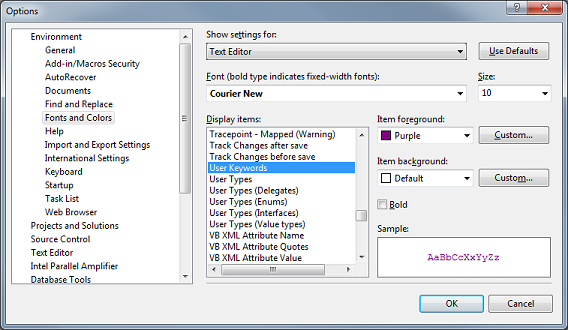
\includegraphics[width=5in]{OptionsDialog.png}
\end{center}

The macro \Code{WM5\_UNUSED(variable)} is used to avoid compiler warnings
iabout unused variables when compiling Release configurations.  For example,
\begin{verbatim}
    bool successful = DoSomeOperation();
    assert(successful);
\end{verbatim}
will compile without warnings in Debug configurations.  However, the
compiler generates a warning in Release configurations that \Code{successful}
is not used.  The reason, of course, is that the \Code{assert} statement has
no generated code in Release configurations, so \Code{successful} is not used.
To avoid the warning, use
\begin{verbatim}
    bool successful = DoSomeOperation();
    assert(successful);
    WM5_UNUSED(successful);
\end{verbatim}

The header file contains three additional blocks, all enabled in Debug
configurations.  The first is related to run-time assertions, the second is
related the WM5 memory management system that supports testing for memory
leaks, and the third is related to file and buffer input-output.  The various
preprocessor commands in these blocks are described later in this document.

\subsubsection{Wm5MathematicsLIB.h}

Currently, the only preprocessor control in \Code{Wm5MathematicsLIB.h} is
related to handling of exact rational arithmetic.  I added a patch to
WM4.10 so that subnormal (denormal) floating-point numbers are handled
correctly by the class \Code{Rational} constructors and converters between
floating-point and \Code{Rational}.  The WM5 code supports conversion of
subnormal numbers.  You can enable the engine to assert when an attempt is
made to convert a NaN (Not a Number) to a \Code{Rational}.

\subsubsection{Wm5GraphicsLIB.h}

A few controls are allowed in \Code{Wm5GraphicsLIB.h}.  When reorienting the
camera by a call to \Code{Camera::SetAxes}, either explicitly or indirectly
with a call to \Code{Camera::SetFrame}, the input axis vectors might be
computed by the application in such a manner that, over time, numerical
round-off errors cause the vectors not to be a right-handed orthonormal set.
The \Code{SetAxis} function uses Gram-Schmidt orthonormalization to ensure
that the vectors do form a right-handed orthonormal set.  You can enable
\Code{WM5\_VALIDATE\_CAMERA\_FRAME\_ONCE} to trap the first time the
vectors appear to fail the test for right-handed orthonormality.  I have
found this to be a useful feature for trapping when the initial settings
for the application camera, \Code{mCamera}, are applied.  In most cases,
the user has incorrectly specified the vectors.

The shader system supports only a few shader models (profiles).  To be
specific, currently only four profiles are supported, but also a {\em none}
value is used to flag invalid profiles.  The total number, including
the {\em none} profile is five. For vertex shaders, the supported profiles
are \Code{vs\_1\_1}, \Code{vs\_2\_0}, and \Code{vs\_3\_0} for DirectX 9 and
\Code{arbvp1} for OpenGL.  For pixel shaders, the supported profiles are
\Code{ps\_1\_1}, \Code{ps\_2\_0}, and \Code{ps\_3\_0} for DirectX 9 and
\Code{arbfp1} for OpenGL.  Sometimes you might need advanced OpenGL support
for an effect, but the Cg compiler still includes the ARB versions of the
profile names in the compiled code.  For example, the sample graphics
application \Code{VertexTextures} requires a Cg command-line parameter
\verb|-profile vp40|, but the Cg compiler still displays the first line
of the compiled file as \verb|!!ARBVP1.0|.  The WM5 shader system bundles
together the shader programs for the profiles into a single object of class
\Code{Shader}.  This class has arrays whose number of elements is 5, which
is stored as \Code{Shader::MAX\_PROFILES}.

{\em You can modify WM5 to include more profiles.}  However, if you use the
WM5 streaming system, the streamed output implicitly depends on
\Code{Shader::MAX\_PROFILES}.  If you were to increase the maximum number
of profiles, and then load a file streamed with the previous maximum number,
there is a mismatch and the file load will ungracefully fail (all data loaded
thereafter is misaligned).  To trap this problem when loading files, you can
enable \Code{WM5\_ASSERT\_ON\_CHANGED\_MAX\_PROFILES}.

In the \Code{Renderer::Draw(const Visual*, const VisualEffectInstance*)}
function, the global render state is reset to the defaults after each pass
of the effect.  Given that every draw function is required to set the
all the global state, it is not necessary to reset the state.  Thus, the
reset code is not compiled by default.  During development and testing, I
had some problems when not resetting the state, so I added a preprocessor
symbol to allow me to toggle the reset code:
\Code{WM5\_RESET\_STATE\_AFTER\_DRAW}.  Just in case problems show up later,
I kept the preprocessor symbol.  You can enable this if you prefer by
uncommenting the define in \Code{Wm5GraphicsLIB.h}.

Sometimes during application development, you might not see a rendered
object when you were expecting one.  A simple test to determine whether
any pixels were actually drawn involves queries supported by the graphics
APIs.  The \Code{Renderer::DrawPrimitive} calls in \Code{Wm5Dx9Renderer.cpp}
and \Code{Wm5OpenGLRenderer.cpp} have conditionally compiled blocks of
code that, when enabled, perform the queries.  To enable these, uncomment
the \Code{WM5\_QUERY\_PIXEL\_COUNT} symbol in \Code{Wm5GraphicsLIB.h}.
Recompile the graphics library and your application, and then set a
breakpoint in \Code{DrawPrimitive} on the lines with \Code{WM5\_END\_QUERY}.
When you reach the breakpoint, step over the line of code and look at the
value of \Code{numPixelsDrawn}.  If it is zero, no pixels were drawn for
the current primitive.

When using the OpenGL renderer, I have code to draw text either using
display lists or using precomputed bitmap fonts (see
\Code{Wm5GLVerdanaS16B0I0.cpp}).  The default is to use display lists,
but you can change this by commenting out \Code{WM5\_USE\_TEXT\_DISPLAY\_LIST}
in \Code{Wm5GraphicsLIB.h}.

\Code{Wm5GraphicsLIB.h} contains the symbol
\Code{WM5\_USE\_OPENGL2\_NORMAL\_ATTRIBUTES} that is defined for Microsoft
Windows and Linux.  It is not defined for Macintosh OS X.  I had problems
with incorrent renderings on the Macintosh when the effects use lighting
and normals, so I had to fall back to using the conventional
\Code{glNormalPointer} for setting the vertex data source for normals.
As it turns out, the problem is that I have been using OpenGL extensions
for shader support, and those extensions were created before OpenGL 2.0
was released.  The assembly for the compiled shaders contains
\Code{vertex.normal}, which is for the conventional way of accessing
the vertex normals.  When I use \Code{glEnableVertexAttribArrayARB}
and \Code{glVertexAttribPointerARB} to set the data source for vertex
normals, the NVIDIA drivers for Microsoft Windows and for Fedora Linux
hook up the normals so that \Code{vertex.normal} refers to those normals.
However, the NVIDIA drivers on the Macintosh do not hook these up, so
the vertex shader is unable to access the normals.

I added the aforementioned preprocessor symbol as a hack to make the shaders
work on all platforms.  Alternatively, on the Macintosh you can edit the
assembly code and replace \Code{vertex.normal} by the corresponding
generic attribute accessor (not my first choice).  I am in the process
of updating the OpenGL renderer so that it uses the core OpenGL 2.0 (and
later) shader system.  However, this means that the shaders must be written
in GLSL, not in Cg.  The end result of the update is {\em EmeraldGL}, and
will be an OpenGL-only graphics system.  I might consider implementing
a DirectX-only system ({\em EmeraldDX}) that uses DirectX 11.

The last preprocessor symbol in \Code{Wm5GraphicsLIB.h} is
\Code{WM5\_PDR\_DEBUG}, which is enabled by default for the DirectX 9
renderer.  This exposes assertions that are triggered whenever the DirectX
calls fail.

\subsubsection{Wm5PhysicsLIB.h}

The only preprocessor symbols in \Code{Wm5PhysicsLIB.h} are used for debugging
the LCP code.  There is no reason to enable these except if you want to
determine whether the LCP code is working correctly.  The LCP code was
part of {\em Game Physics, 1st edition}, but it was intended to be pedagogic
and illustrate the Lemke algorithm (which looks a lot like a basic linear
programming solver and similar to linear system solving).  This code is not
what people use in physics engines.  (Someday I will get around to implementing
a velocity-based iterative algorithm \ldots)

\subsubsection{Wm5ImagicsLIB.h}

No preprocessor symbols are defined in \Code{Wm5ImagicsLIB.h}.  This library
has not been worked on for many years, but remains useful (to me) for rapid
prototyping of image analysis projects.  It needs some major updating and
expansion.


\subsection{No DLL Configurations}

For years I have provided build configurations for both static and dynamic
libraries.  The Microsoft Windows annoyance of having to use
\Code{\_\_declspec(dllexport)} and \Code{\_\_declspec(dllimport)} so that
classes are properly exported or imported has been a pain.  The WM4
libraries had LIB files containing preprocessor symbols as shown next:
\begin{verbatim}
    #ifdef WM4_FOUNDATION_DLL_EXPORT
        // For the DLL library.
        #define WM4_FOUNDATION_ITEM __declspec(dllexport)
    #else
        #ifdef WM4_FOUNDATION_DLL_IMPORT
            // For a client of the DLL library.
            #define WM4_FOUNDATION_ITEM __declspec(dllimport)
        #else
            // For the static library.
            #define WM4_FOUNDATION_ITEM
        #endif
    #endif
\end{verbatim}
Each class is structured as
\begin{verbatim}
    class WM4_FOUNDATION_ITEM MyClass { ... }
\end{verbatim}
However, template classes with no explicit instantiation in the library
could not use the \Code{WM4\_FOUNDATION\_ITEM} macro.  And various
static class data members needed the macro per member.  The separation
between the abstract \Code{Renderer} class and its derived classes per
graphics API required the virtual function members so that the DLL configurations
would link successfully.

Given the abundance of disk space, the usage I had in mind for Wild Magic
libraries, the problems with linking when attempting to remove virtual
functions from the \Code{Renderer} class, and the annoyance of the
aforementioned macro handling, I decided to stop supporting DLLs.  WM5 has
only static debug and static release configurations.

\subsection{The WM4 Shader Programming and FX System}

WM4 had a somewhat complicated approach to shader programming and effects,
which made it sometimes difficult to extend to shaders not already part of
the engine (or part of the sample applications).  The problems with this
approach are described next.

The abstraction of the drawing pass in WM4 is

\scriptsize
\begin{verbatim}
    renderer.Draw(geometry)
    {
        renderer.SetGlobalState(...);  // alpha, cull, depth, ...
        renderer.SetWorldTransformation();  // sets model-to-world (W), others computed later (WV, WVP)
        renderer.EnableIBuffer(geometry);  // enable the index buffer of geometry
        for each effect of geometry do // multieffect drawing loop
        {
            renderer.ApplyEffect(effect);
            {
                for each pass of effect do  // multipass drawing loop
                {
                    pass.SetGlobalState();
                    pass.ConnectVShaderConstants();  // set sources for constants
                    pass.ConnectPShaderConstants();  // set sources for constants
                    pass.GetVProgram();  // loaded first time, cached in catalog for later times
                    pass.EnableVProgram();
                    pass.GetPProgram();  // loaded first time, cached in catalog for later times
                    pass.EnablePProgram();
                    for each vertex texture of pass do
                    {
                        pass.GetVTexture();  // loaded first time, cached in catalog for later times
                        pass.EnableVTexture();
                    }
                    for each pixel texture of pass do
                    {
                        pass.GetPTexture();  // loaded first time, cached in catalog for later times
                        pass.EnablePTexture();
                    }
                    pass.EnableVBuffer();
                    renderer.DrawPrimitive(geometry);
                    pass.DisableVBuffer();
                    pass.DisablePTextures();
                    pass.DisableVTextures();
                    pass.DisablePProgram();
                    pass.DisableVProgram();
                    pass.RestoreGlobalState();
                }
            }
        }
        DisableIBuffer();
        RestoreWorldTransformation();
        RestoreGlobalState();
    }
\end{verbatim}
\normalsize

The drawing supports multiple effects per geometric primitive and multiple
passes per effect; it is not necessary to have a double-loop sytem.  WM5
has a single-loop system, iterating over the passes of a single effect
attached to the geometric primitive.

The renderer sets and restores global states (alpha, face culling, depth
buffering, stencil buffering, polygon offset, wireframe), but so does each
pass.  Given that each pass restores state, there is no need for the renderer
object itself to manage global state.

The index buffer is invariant across all effects and passes, so it is enabled
and disabled once only.  However, the vertex buffer is enabled and disabled
per pass, which is not necessary.  What WM4 does is create a VRAM vertex
buffer for the geometric primitive.  It then maintains vertex buffers
that match what the vertex program requires for the passes, as determined
during the first call to \Code{GetVProgram} (when the vertex program is
loaded from disk and parsed).  If the effect has multiple passes, a second
(or later) pass involves finding an already existing vertex buffer that has
the required attributes.  If none exists, a new VRAM vertex buffer is created
that has the required attributes.  Thus, it is possible that multiple vertex
buffers exist in VRAM with data copied from the primary vertex buffer of the
geometric primitive, which is a waste of memory.  An effect with multiple
passes should be applied to a geometric primitive whose vertex buffer has
{\em all} the attributes necessary for {\em all} the passes (WM5 does this).

In effect, WM4 tried to assume responsibility for ensuring that the vertex
buffers match what the vertex program needs.  If there is a mismatch between
primary vertex buffer and what the vertex program needs, WM4 creates a
matching vertex buffer; however, the attributes generated by a mismatch have
have no chance of being initialized by the application programmer.  In the
WM4 sample applications, there are no mismatches, so there is no penalty in
wasted memory.  But there is a penalty in having a vertex buffer management
system that is irrelevant.  In the end, it is the application programmer's
responsibility for ensuring that the vertex buffer has all that it needs to
support an effect and that the outputs of a vertex program match the inputs
of a pixel program.

In WM4, class \Code{Shader} represents a shader program and its associated
storage for shader constants and for textures.  However, it was convenient
to allow applications to specify their own data sources for the shader
constants (for ease of access).  WM4 has shader constant classes that
provide such storage; for example, the class \Code{UserConstant}.  In the
drawing pass, the functions \Code{Renderer::ConnectVShaderConstants} and
\Code{Renderer::ConnectPShaderConstants} set the data sources for the
shaders.  This allows an application to change the data source for each
drawing pass, an event that is highly unlikely (and never happens in WM4
sample applications).  The redesign of the shader system for WM5 avoids
this.

The function \Code{Renderer::GetVProgram} is called during drawing to
get access to the vertex program of the effect pass.  The first time a
vertex program is requested, it is loaded from disk.  The shaders were
written using NVIDIA's Cg, and they were all compiled for Shader Model 2.
The compiled assembly is still textual, and is stored in files with
extension \Code{wmsp}.  The WM4 engine contains a class \Code{Program}
and derived classes \Code{VertexProgram} (loads \Code{wmsp} files with
prefix \Code{v\_}) and \Code{PixelProgram} (loads \Code{wmsp} files with
prefix \Code{p\_}).  The comments in the \Code{wmsp} files are parsed
to obtain information about the shader program, which effectively is
WM4's attempt to have an FX run-time system.

A problem with this system is that the shader programs are constrained
to contain special names for some of the shader constants to support
automatic updating of those constants during drawing.  A class
\Code{RendererConstant} provides a set of enumerations and corresponding
names for common quantities that change frequently, such as
world-view-projection matrices, camera parameters, and light and
material parameters.  Class \Code{Renderer} contains an array of functions
corresponding to the enumerations in \Code{RendererConstant}.  The
function \Code{Renderer::SetRendererConstant} determines which shader
constants need to be updated (in system memory).  After such a call,
\Code{Renderer::SetVProgramConstant} or \Code{Renderer::SetPProgramConstant}
are called so that the graphics API can update the constants (by copying
to constant registers).  These \Code{Renderer} calls are part of the
\Code{Renderer::EnableVProgram} and \Code{Renderer::EnablePProgram} calls
in the drawing pass.  WM5 provides a different mechanism for automatic
constant updating that does not have constraints on the shader constant
names.

Another problem with the \Code{Program} loading and parsing is that it
is not general.  Often I would want to support a new effect but the
Cg programs used features not supported by the parser of
\Code{Program}.  That meant modifying \Code{Program} as needed.  WM5
avoids this system and allows you to compile shaders to a binary format
that contains the textual program string but also contains information
about the shader.  That is, the loading and parsing is now part of a
tool.  The output files of the tool are ready to load by WM5, so there
is no error checking that needs to be performed at application run time.

In WM4, when \Code{Renderer::GetVProgram} is called the first time for a
vertex program, and the program loads correctly, it is stored in a cache
implemented in the \Code{Catalog} class.  This caching system is overly
complicated.  In WM5, caching is the responsibility of the application
programmer, because the programmer knows best how the objects will be
used and shared.

When effects use vertex or pixel textures, they are loaded the first time
they are encountered by calls to \Code{ShaderEffect::GetVTexture} and
\Code{ShaderEffect::GetPTexture}.  The mechanism is similar to that of
\Code{GetVProgram} and \Code{GetPProgram}--the first time a texture is
encountered, it is loaded from disk and cached in a catalog.  Later
requests look in the catalog first to find the textures and, if found,
use them instead of loading a new copy from disk.

Although manageable, the drawing system of WM4 turned out to be more
complicated than is necessary, and it was not general enough to support
many advanced special effects without having to modify the engine.

\subsection{The WM5 Shader Programming and FX System}
\label{subsec.shaderfx}

The abstraction of the drawing pass in WM5 is described next.  What used
to be the \Code{Geometry} class is now \Code{Visual}, which I thought
was a better name that allows me to add \Code{Audial} (for 3D sound) at
a later date.

Some other major design changes were made.  DirectX 9 has the concept of
a {\em vertex format} that describes a vertex stored in a vertex buffer.
OpenGL does not encapsulate this in a simple manner.  WM5 has a new class
called \Code{VertexFormat} that implements the idea.  The class
\Code{VertexBuffer} still represents a vertex buffer but, of course, with
changes.  Reading and writing vertex buffer information requires knowing
a vertex buffer and a vertex format.  The read/write is supported by the
class \Code{VertexBufferAccessor}.

The WM5 class \Code{VisualEffect} is the natural successor to WM4's
\Code{ShaderEffect}, except that \Code{VisualEffect} represents a
vertex shader and pixel shader pair {\em but without specific data for
the shader constants and textures}.  A single \Code{VisualEffect} object
can have multiple instances, each instance having data.  These instances
are represented by class \Code{VisualEffectInstance}.  For example, you
can create a texture visual effect with user-specified sampler parameters.
If you want this effect for each of two different texture images, you
create two visual effect instances.

A \Code{Visual} object has attached a single pair of \Code{VisualEffect}
and \Code{VisualEffectInstance}.  Each object of type \Code{VisualEffectInstance}
manages multiple passes for the drawing, each pass of class \Code{VisualPass}.
The \Code{VisualPass} class contains global render state objects (alpha,
face culling, depth buffering, polygon offset, stencil buffering, and
wireframe), a vertex shader, and a pixel shader.

A class \Code{ShaderParameters} represents the shader constants and
textures used \Code{VisualEffectInstance}, one such object for the
vertex shader and one such object for the pixel shader.  The shader
constants are encapsulated by a system whose base class is \Code{ShaderFloat}.
Many derived classes are provided for common shader constants, such as
world-view-projection matrices, camera parameters, and light and material
parameters.  This system replaces WM4's \Code{RendererConstant} system for
automatic updating of shader constants.

The drawing pass is abstractly

\scriptsize
\begin{verbatim}
    renderer.Draw(visual, visualEffectInstance)
    {
        renderer.Enable(visual.vertexBuffer);
        renderer.Enable(visual.vertexFormat);
        renderer.Enable(visual.indexBuffer);  // if it has such a buffer
        for each visualPass of visualEffectInstance do
        {
            visualPass.vertexShaderParameters.UpdateConstants(visual, renderer.camera);
            visualPass.pixelShaderParameters.UpdateConstants(visual, renderer.camera);
            visualPass.SetGlobalState();  // alpha, cull, depth, ...
            renderer.Enable(visualPass.vertexShader, visualPass.vertexShaderParameters);
            renderer.Enable(visualPass.pixelShader, visualPass.pixelShaderParameters);
            renderer.DrawPrimitive(visual);
            renderer.Disable(visualPass.pixelShader, visualPass.pixelShaderParameters);
            renderer.Disable(visualPass.vertexShader, visualPass.vertexShaderParameters);
            visualPass.RestoreGlobalState();
        }
        renderer.Disable(visual.indexBuffer);
        renderer.Disable(visual.vertexFormat);
        renderer.Disable(visual.vertexBuffer);
    }
\end{verbatim}
\normalsize

At a high level, the drawing is similar to that of WM4.  But as mentioned in the
section describing the WM4 drawing, the vertex buffer is enabled and disabled once
outside the loop over passes.  The WM4 setting of sources for shader constants was
eliminated.  Instead, the \Code{ShaderFloat} objects provide storage and the
\Code{UpdateConstants} performs the automatic updates of the constants.

All caching of effects, textures, vertex buffers, vertex formats, and index buffers
is the responsibility of the application programmer.  It is simple enough to use
the smart-pointer system for the management rather than a complicated cataloging
system.

As mentioned in the previous section, WM5 has a tool for compiling Cg Shaders
to a binary format that can be loaded directly by the engine.  This tool is
named \Code{WmfxCompiler} (in the \Code{WildMagic5/Tools} subfolder).

{\em Local effects} are those applied to a single geometric primitive; for
example, basic texturing and lighting.  {\em Global effects} are typically more
complicated and are applied to scene graphs; for example, planar shadows and
planar reflections.  WM5 has implementations of quite a few local effects, but
has only planar shadows and planar reflections as examples of global effects.
The sample applications have additional global effects that are implemented at
the application level rather than as classes.

\subsection{Design Change Regarding Lights and Materials}
\label{subsec.designchangelights}

WM4 had classes \Code{Light} and \Code{Material} that provided the ability to
attach \Code{Light} objects to a scene graph node.  Each light attached to a
node was assumed to illuminate any objects in the subtree rooted at the node.
To support this automatically, WM4 internally generated a shader effect
(class \Code{LightingEffect}) that was used for lighting.  If an application
attached a \Code{ShaderEffect} to a leaf node of that subtree, a multieffect
drawing occurred.  The \Code{LightingEffect} was executed first for
the geometry, and the \Code{ShaderEffect} was executed second with a default
alpha blend applied to combine it with the lighting.  This approach still
has the flavor of the fixed-function pipeline.  Moreover, it was not a good
idea (based on technical support requests from users having problems working
with the lighting).  It is possible to roll your own lighting effects without
attaching lights to the scene, but then you have to make \Code{Renderer} calls
so that the renderer knows about the lights.  Very cumbersome and nonintuitive.

WM5 eliminates this system.  The \Code{Light} class still exists, but it is
only a container for light properties (light type, colors, attenuation, and
so on).  You cannot attach a \Code{Light} to a scene directly.  Instead, you
can create lighting-related shader constants via classes derived from
\Code{ShaderFloat} and include them in the visual effect instances.  See,
for example, files of the form \Code{Wm5Light*Constant.\{h,cpp\}} and
\Code{Wm5Material*Constant.\{h,cpp\}} and local effects files of the form
\Code{Wm5Light*Effect.\{h,cpp\}}.

\section{LibCore}

The \Code{LibCore} library contains some basic support that applications need.
Some of this support is for convenience during development.  A summary of
the files in this library is provided in this section.  The subsection titles
are the names of the subfolders of the \Code{WildMagic5/LibCore} folder.

\subsection{Assert}

C$++$ run-time libraries typically implement a macro called \Code{assert}
that has a single input which is a Boolean expression.  In debug
configurations, the macro is expanded to platform-specific code that triggers
the assertion when the Boolean expression is false.  Moreover, typically
a breakpoint is generated so that the debugger stops on that line of code
for the programmer to diagnose the problem.  For example,
\begin{verbatim}
    float numerator = <some integer>;
    float denominator = <some integer>;
    assert(denominator != 0.0f);
    float ratio = numerator/denominator;
\end{verbatim}
This bare-bones approach is suitable most of the time, but other times it
is useful to perform more actions when an unexpected condition occurs.
Moreover, it might be useful to have an assertion triggered when running
in release configurations.

The files \Code{Wm5Assert.*} provide an alternate implementation for
assertions, which at the moment is utilized only on Microsoft Windows
and Microsoft Visual Studio.  The class \Code{Assert} has a constructor whose
first input is the Boolean expression to be tested.  The name of the file and
line number within that file where the assertion is triggered are also
parameters.  These support writing assertions to a logfile, identifying
the file and line number, but not triggering an interrupt on the assertion.
These also support writing information to a Microsoft Windows message box.

Yet another parameter of the constructor is a format string.  Values to be
printed via the format statement may be provided to the constructor (note
the use of the ellipsis in the constructor).  This allows you to specify
more than just that the assertion failed.  You can print as much information
as you believe necessary to help with debugging.  A variadic macro named
\Code{assertion} is used to wrap the construction of \Code{Assert} objects;
such a macro supports a variable number of arguments.

By default, the alternative assertion system is enabled for Microsoft
Windows and Visual Studio when in a debug configuration.  The preprocessor
flag controlling this is in \Code{Wm5CoreLIB.h}.  The system is enabled
when \Code{WM5\_USE\_ASSERT} is defined.  If you want, you can expose the
macros even in a release configuration.  Notice that there are three
additional preprocessor symbols you can define.  These control whether
the assertion information is written to a log file, to the output window
of Visual Studio, and/or to a message box.

In my environment, I have \Code{assertion} specified as a user keyword
with syntax highlighting that shows the keyword in purple.  For details
on highlighting user keywords, see Section \ref{subsubsec.corelib}.

\subsection{DataTypes}

I implemented only two basic data types in the core library:  \Code{Tuple}
and \Code{Table}.  These are templated classes with two template
parameters: one is the number of components of the tuple and one is the
type of the component.  Only basic services are provided:  construction,
destruction, access to the array pointer, access to components, assignment,
and comparison (support for standard C$++$ library containers).  The main
use of \Code{Tuple} in the engine is as a base class for floating-point
vectors \Code{Float1}, \Code{Float2}, \Code{Float3}, and \Code{Float4}.
The derived classes provided specialized constructors and assignment
operators.

Class \Code{Table} represents a 2-dimensional array of components and has
three template parameters: one is the number of rows of the table, one is
the number of columns of the table, and one is the type of the component.
Only basic services are provided:  construction, destruction, access to
the array pointer, access to components, access to rows and columns (as
tuples), assignment, and comparison (support for standard C$++$ library
containers).  The main use of \Code{Table} in the engine is as a base
class for floating-point matrices \Code{Matrix2}, \Code{Matrix3}, and
\Code{Matrix4}.

I have tried to rely on the standard C$++$ library containers as much as
possible, but I find my own minimum-heap template class to be useful (for
priority queue support with fast updates when neighbors change).  I have
kept this template class, files \Code{Wm5MinHeap.*}.

\subsection{InputOutput}

This folder contains implementation for handling of byte-order (endianness)
and for file and buffer input-output.  It also contains a path system for
locating files.

\subsubsection{Endianness}

Class \Code{Endian} has code to test whether a processor is little endian
or big endian.  The class also has functions for swapping data types with
2, 4, or 8 bytes per element.  I used byte-swapping in WM4 extensively to
allow data files that could be loaded either on a little-endian or a
big-endian machine.  The data itself was always stored in little-endian
format, which meant that the PowerPC Macintosh had extra computational
work to do when loading.

\subsubsection{File and Buffer Input-Output}

My goal in WM5 was to provide file and buffer input-output that can be
configured for the platforms in such a manner as to avoid byte swapping.
Classes \Code{BufferIO} and \Code{FileIO} are the implementations.  The
constructors for these classes have a \Code{mode} parameter that allows
you to specify whether the object is for reading data or for writing
data.  Moreover, the \Code{mode} flags specify whether to read as is,
to write as is, to read and swap bytes, or to write and swap bytes.
Additionally, I have \Code{mode} flags for the default read/write modes.
In the engine, any time I use \Code{BufferIO} or \Code{FileIO} objects,
I arrange for the \Code{mode} parameter to be defaulted itself to the
default read/write modes.  In this manner, if you want a global change
in the engine, say, to switch from read to read-and-swap, you need only
edit \Code{Wm5BufferIO.h} and \Code{Wm5FileIO.h} and change what the
default flags are (they currently are set to read/write without swaps).

This sounds fine in theory, but I encountered one big problem after
writing most of the graphics library.  The vertex buffers and textures
were streamed to disk as arrays of bytes, ignoring the actual structure
of a vertex and the actual format of a texture.  This is a problem when
you want to write-and-swap, because byte arrays are never byte-swapped.
Instead, it is necessary to write vertices one at a time and swap native
fields as they are encountered.  Similary, texels must be written one at
a time to ensure that the color channels are swapped correctly; for
example, if you have an RGBA 16-bits-per-channel texel, you must swap
two bytes per channel for each of four channels.  The source code was
due soon for the {\em Game Physics, 2nd edition} CD-ROM, so it was too
late to modify the code.  Instead, I created WMOF (Wild Magic Object
File) versions for little endian and big endian.  Only two such files
are shipped anyway (\Code{FacePN.wmof} and \Code{SkinnedBipedPN.wmof}),
so not a big deal.  My goal for future development is to avoid the
streaming system and just rely on raw formats for vertex buffers,
index buffers, and textures, and each platform can generate its own
byte-ordered versions.

\subsubsection{Path Handling}

In WM4, the files \Code{Wm4System.*} contained the ability to specify
a filename and create the fully qualified hard-disk path for the file.
The function of interest was \Code{System::GetPath}.  Someone who had
experience with the Macintosh implemented the Apple version of this
function, which involves some low-level operating system calls.  I
had to hack this function, because it depended on how Xcode was
configured (and the configuration varied between Xcode versions).
Not having enough experience with low-level Macintosh programming,
I ignored some complaints from users about how \Code{GetPath} was
slow and annoying.

In WM4, I also required users to set an environment variable that
stored the path to the \Code{WildMagic4} folder of the installation.
I missed a simple opportunity to bootstrap off this environment
variable and avoid the low-level programming.

WM5 does take advantage of the environment variable, now called
\Code{WM5\_PATH} in the WM5 distribution.  Class \Code{Environment}
encapsulates computing the fully qualified path for a specified file.
Just as class \Code{System} allowed in WM4, \Code{Environment}
allows you to insert and remove directory strings (paths to the
folders) for an array of strings.  The most common function in this
class that the sample applications use is
\begin{verbatim}
    std::string Environment::GetPathR (const std::string& name);
\end{verbatim}
You specify the name of a file to be read (the suffix \Code{R}
stands for ``read'') and the function returns the fully qualified
path for that file, if it can find it using the array of directory
strings it manages.  If it cannot find the function, the empty
string is returned.

The main entry point in the application code inserts the path to
the \Code{WildMagic5} folder.  It also inserts paths to various
\Code{WildMagic5/Data} subfolders: \Code{Wmfx}, \Code{Wmof},
\Code{Wmtf}, \Code{Wmvf}, and \Code{Im}.  More importantly, the
path to the application's project folder is inserted in the
main function.  The application initialization mechanism sets the
path, which is a static member \Code{Application::ThePath}.  In
order for this to work, it is necessary that the application
set the console title (for \Code{ConsoleApplication}-derived
classes) or the window title (for \Code{WindowApplication}-derived
classes).  For example, the application \Code{BillboardNodes}
has a class with constructor defined as
\begin{verbatim}
    BillboardNodes::BillboardNodes ()
        :
        WindowApplication3("SampleGraphics/BillboardNodes",0, 0, 640, 480,
            Float4(0.9f, 0.9f, 0.9f, 1.0f)),
            mTextColor(1.0f, 1.0f, 1.0f, 1.0f)
    {
    }
\end{verbatim}
The window title is the quoted string.  This string is appended to
the fully qualified string for the \Code{WildMagic5} folder.  The
resulting string is the fully qualified path for the folder of the
\Code{BillboardNodes} project.

\subsection{Memory}

\subsubsection{WM4 Memory Tracking}

WM4 has a memory system that supported finding memory leaks.  The macros
\Code{WM4\_NEW} and \Code{WM4\_DELETE} are simple macros that wrap
\Code{new} and \Code{delete} when the memory system is disabled and
that wrap \Code{new(\_\_FILE\_\_,\_\_LINE\_\_)} and \Code{delete} when the
memory system is enabled.  All engine memory allocations and
deallocations use these macros so that without code changes, you can
toggle on/off the memory tracking.

The heart of the system is class \Code{Memory} whose interface is used
to override the C$++$ operators
\begin{verbatim}
    void* operator new (size_t size, char* file, unsigned int line);
    void* operator new[] (size_t size, char* file, unsigned int line);
\end{verbatim}
Although a simple system, the override affects all allocations in the
application; indirectly, any other code linked to the application is
forced to use the overridden operator.

I was not satisfied with this approach, wanting instead to provide the
ability for users to substitute in their own memory management/tracking
system that affects only Wild Magic code.  For example, a user might want
to patch in a system that gives Wild Magic a {\em memory budget}--a
fixed-size heap that the engine must use for all its memory needs.

I also was not satisfied with the C$++$ memory management itself.  In
the memory tracking, the calls to \Code{new(\_\_FILE\_\_,\_\_LINE\_\_)}
allow you to intercept the allocation request and save it for writing
to a log file at the end of an application run.  If there is a memory
leak, the log file can list information about the allocations, including
the name of the source file and the line of that file where the leaked
allocation occurred.  Unfortunately, C$++$ does not allow you to override
\Code{delete} in a way that uses the \Code{\_\_FILE\_\_} and
\Code{\_\_LINE\_\_} macros.  At first glance you might override with
\begin{verbatim}
    void operator delete (void* address, char* file, unsigned int line);
    void operator delete[] (void* address, char* file, unsigned int line);
    #define WM4_DELETE delete(__FILE__,__LINE__)
\end{verbatim}
This does not do what you think it does.  These versions of \Code{delete}
are called only when exceptions occur, and you cannot force them to be
called otherwise.  It would really be helpful to be able to log the files
and lines on which deallocations occur, especially when you want to monitor
{\em memory usage patterns} rather than memory leaks.

The \Code{operator new} function is for dynamically allocating a single object,
a 0-dimensional array so to speak.  The \Code{operator new[]} function is for
dynamically allocating a 1-dimensional array of objects.  The general rule is
that if you allocate with \Code{operator new}, you must deallocate with
\Code{operator delete}.  If you allocate with \Code{operator new[]}, you must
deallocate with \Code{operator delete[]}.  If you mix these, consider that
an error in memory management, even if the application does not abnormally
terminate.  For example,
\begin{verbatim}
    MyObject* objects = new MyObjects[10];
    delete[] objects;  // matches the new[] call
    delete objects;  // error - a mismatch
\end{verbatim}
It is the programmers reponsibility to ensure the new and delete calls are
matched.

C$++$ does not have new/delete operators for higher dimensional arrays.  It is
not clear how to provide language support for this in a robust manner.  For
example,
\begin{verbatim}
    MyObject** objects0 = new MyObject*[N];
    for (i = 0; i < N; ++i)
    {
        objects0[i] = new MyObject[M];
    }
    <code using objects0>;
    for (i = 0; i < N; ++i)
    {
        delete[] objects0[i];
    }
    delete[] objects0;
    
    MyObject someObjects[N];  // objects live on the stack, not in the heap
    MyObject** objects1 = new MyObject*[N];
    for (i = 0; i < N; ++i)
    {
        objects0[i] = &someObjects[i];
    }
    <code using objects1>;
    delete[] objects1;
\end{verbatim}
In the first block of code, the user has dynamically allocated a 2-dimensional
array of \Code{MyObject} objects, manipulated the objects, and then dynamically
deallocated the array one row at a time.  In the second block of code, the
user has created a 1-dimensional array of \Code{MyObject*} pointers that
point to a 1-dimensional array of \Code{MyObject} objects that live on the
stack.  It is an error to attempt to dynamically deallocate these objects.
Clearly, the semantics of \Code{objects0} and \Code{objects1} are different,
despite both being of type \Code{MyObject**}.  Without knowledge of the
semantics, it would be difficult for C$++$ to provide a new/delete pair
for \Code{Type**} pointers.

In the case when the user does want a 2-dimensional array of the form
that \Code{objects0} illustrates, you can provide your own allocation
and deallocation.  WM4 had several template functions in class \Code{System}
for allocating and deallocating 2-dimensional and 3-dimensional arrays.
The idea of these is to encapsulate the work required, hiding the details
from the user, {\em and to minimize the number of new/delete calls}.
Returning to the first code block of the example, an alternative scheme
that minimizes new/delete calls is
\begin{verbatim}
    MyObject* objects2 = new MyObject*[N];
    objects2[0] = new MyObject[N*M];
    for (i = 1; i < N; ++i)
    {
        objects2[i] = &objects2[0][M*i];
    }
    <code using objects2>;
    delete[] objects2[0];
    delete[] objects2;
\end{verbatim}
Allocation of \Code{objects0} requires $N+1$ calls to \Code{new} and
deallocation requires $N+1$ calls to \Code{delete}.  Allocation of
\Code{objects2} requires $2$ calls to \Code{new} and $2$ calls to
\Code{delete}.  Calls to new/delete can be relatively expensive because
of the work that the memory manager must due to manage the free list of
blocks, so minimizing the calls is a desirable goal.  Moreover, you are
guaranteed that the \Code{N*M} \Code{MyObject} objects are contiguous,
which can be friendly to a memory cache, and also allows you to iterate
over the 2-dimensional array as a 1-dimensional array in an efficient
manner.
\begin{verbatim}
    // Iteration as a 2-dimensional array.
    for (row = 0; row < N; ++row)
    {
        for (col = 0; col < M; ++col)
        {
            MyObject& object = objects2[row][col];
            <do something with object>;
        }
    }
    
    // Iteration as a 1-dimensional array.
    for (i = 0; i < N*M; ++i)
    {
        MyObject& object = objects[0][i];
        <do something with object>;
    }
\end{verbatim}
In the memory allocation scheme for \Code{objects2}, you are not
guaranteed that the rows occur in contiguous memory, so there is
the potential for memory cache misses when iterating over the
2-dimensional array, and it is not possible to iterate over the
objects as a 1-dimensional array.

Allocation and deallocation of 3-dimensional arrays with a minimum
of new/delete calls is similar.
\begin{verbatim}
    MyObject*** objects3 = new MyObject**[P];
    objects3[0] = new MyObject*[P*N];
    objects3[0][0] = new MyObject[P*N*M];
    for (int j = 0; j < P; j++)
    {
        objects3[j] = &objects3[0][N*j];
        for (int i = 0; i < N; i++)
        {
            objects3[j][i] = &objects3[0][0][M*(i + N*j)];
        }
    }
    <code using objects>;
    delete[] objects3[0][0];
    delete[] objects3[0];
    delete[] objects3;
\end{verbatim}

In WM4, the allocation and deallocation are wrapped with template functions
named \Code{System::Allocate} and \Code{System::Deallocate}.  However, I find
it displeasing to have inconsistent readability by calling \Code{WM4\_NEW}
for single objects (0-dimensional) and 1-dimensional arrays but having to
call \Code{System::Allocate} for 2-dimensional and 3-dimensional arrays.

\subsubsection{WM5 Memory Tracking}

A review of the ideas in the previous section led me to the following
requirements for the WM5 memory management system.  Several additional
requirements were added as I discovered problems while developing the
memory manager.  The first item in the list is about memory tracking
disabled.  All other items are about memory tracking enabled.
\begin{enumerate}
  \item When memory tracking is disabled, the allocation and deallocation
    fall back to the standard \Code{new} and \Code{delete} calls.
  \item Support semantics for arrays of dimension two or larger.
  \item Interception of \Code{new} and \Code{delete} calls must affect
    only the Wild Magic source code; that is, a side effect should not
    be that other systems (C$++$ run-time libraries or third-party
    software) are forced to use the interception system.
  \item Provide hooks to the users for the low-level allocation and
    deallocation so that Wild Magic transparently accesses a user-specified
    heap (to enforce a memory budget).
  \item File names and line numbers must be tracked both for allocations
    and deallocations.
  \item The inclusion of \Code{\_\_FILE\_\_} and \Code{\_\_LINE\_\_}
    macros must be hidden from the user (for readability).
  \item The tracking system must be reentrant; that is, if the system
    manages containers that store tracking information and those
    containers must be dynamically allocated, they must not do so by
    using the tracking system (infinite recursion problem).
  \item The system must allow for smart pointers (reference-counted
    objects).
  \item The tracking system must be thread safe.
\end{enumerate}
I struggled with designing a system that satisfied all the requirements,
finally settling on the one that is implemented in class \Code{Memory}.
I was burned only a couple of times along the way \ldots

\vspace*{0.1in}
{\bf Usage}

Before discussing the issues in designing \Code{Memory}, let us look at
the final result and how it is used.  A set of macros are defined to
make allocation and deallocation calls simple, readable, and that hide
the file-line information.  The allocation macros are named:  \Code{new0},
\Code{new1}, \Code{new2}, \Code{new3}, and \Code{new4}.  The numeric
suffix denotes the dimension of the allocation.  Effectively, \Code{new0}
corresponds to \Code{new} for a single object, \Code{new1} corresponds
to \Code{new[]} for a 1-dimensional array of objects, and the remaining
macros correspond to higher dimensional arrays, as described in the
previous section (minimizing the number of calls to \Code{new}).  The
corresponding deallocation macros are \Code{delete0}, \Code{delete1},
\Code{delete2}, \Code{delete3}, and \Code{delete4}.  Although it is
still the user's responsibility to pair the correct new/delete macro
calls, if there is a mismatch (on a delete call), the memory tracking
system will report this.  In my development environment, these macros
were added as user keywords, which I highlight in purple.

For allocation, all but the \Code{new0} call are templated.  Typical usage is
\begin{verbatim}
    MyObject* object = new0 MyObject(parameters);
    delete0(object);
    
    MyObject* objects1 = new1<MyObject>(numElements);
    objects1[elementIndex] = <do something>;
    delete1(objects1);
    
    MyObject** objects2 = new2<MyObject>(numRows, numColumns);
    objects2[rowIndex][columnIndex] = <do something>;
    delete2(objects2);
    
    MyObject*** objects3 = new3<MyObject(numSlices, numRows, numColumns);
    objects3[sliceIndex][rowIndex][columnIndex] = <do something>;
    delete3(objects3);
\end{verbatim}

\vspace*{0.1in}
{\bf Design Issues}

Now for design issues.  One of the main problems I had was trying to wrap
the allocation and deallocation with macros for readability and ease of
use, yet satisfying all the requirements I mentioned previously.  It
appeared to be practically impossible to use macros, hide an overload
of \Code{operator new} specific to Wild Magic, interact properly with
\Code{new} for single objects, hide the \Code{\_\_FILE\_\_} and
\Code{\_\_LINE\_\_} macros, and fall back to standard \Code{new} and
\Code{delete} when the tracking is disabled.  Moreover, Requirement 7
is problematic, because it effectively forces you to have a container
external to the WM5 memory management system, which means a memory budget
cannot be fully enforced.  I decided that having such a container was
something I (and users) can live with--you can always estimate how large
a container will be for your application, and then factor that into your
memory budgets.

In WM4, I had a macro to wrap overloaded \Code{operator new},
\begin{verbatim}
    #define WM4_NEW new(__FILE__,__LINE__)
    void* operator new (size_t size, char* file, unsigned int line);
    void* operator new[] (size_t size, char* file, unsigned int line);
\end{verbatim}
This macro hides the \Code{\_\_FILE\_\_} and \Code{\_\_LINE\_\_} macros,
satisfying Requirement 6.  However, the overloaded allocators violate
Requirement 3--the compiler would generate code for non-Wild-Magic code
that use the overloads.  Regardless, such a simple macro cannot simultaneously
hide the file-line macros, the dimension of the array to be allocated, and
wrap the overloaded \Code{new}.

I was able to accomplish some of the hiding, but suffered the consequence of
needing lines of code such as
\begin{verbatim}
    MyObject* object = WM5_NEW(MyObject, constructorParameters WM5_FILE_LINE);
\end{verbatim}
where \Code{WM5\_FILE\_LINE} expanded to nothing when memory tracking was
disabled, but expanded to
\begin{verbatim}
    #define WM5_FILE_LINE , __FILE__, __LINE__
\end{verbatim}
when memory tracking was enabled.  I was able to circumvent this problem by
designing \Code{Memory} so that objects of this class were only temporary
(for one line of code) but stored the file-line information.  This also
addressed Requirement 5 (tracking delete calls).  Specifically, class
\Code{Memory} has members \Code{mFile} and \Code{mLine} and a constructor
\begin{verbatim}
    Memory::Memory (const char* file, int line) : mFile(file), mLine(line) { }
\end{verbatim}
The file-line information persists only while the temporary object exists, so
they are temporarily accessible to the memory tracking system.

The overloaded allocation operator has signature
\begin{verbatim}
    void* operator new (size_t numBytes, const Wm5::Memory& memory);
\end{verbatim}
This satisfies Requirement 3 in that it is not possible for the compiler to
match this against allocation calls outside the Wild Magic 5 engine.  There
was no need to overload \Code{operator new[]}.

Some of the macros for allocation and deallocation are
\begin{verbatim}
    #define new0 new(Wm5::Memory(__FILE__,__LINE__))
    #define new1 new Wm5::Memory(__FILE__,__LINE__).New1
    #define delete0 Wm5::Memory(__FILE__,__LINE__).Delete0
    #define delete1 Wm5::Memory(__FILE__,__LINE__).Delete1
\end{verbatim}
Notice that \Code{new0} uses the overloaded \Code{new} operator, where the
input \Code{memory} is a reference to the temporary \Code{Memory} object.
In the implementation of the overloaded \Code{new} operator, the memory
tracking system has access to file-line information because the temporary
object stores that information.

\vspace*{0.1in}
{\bf Template and Macro Interaction}

Notice that \Code{new1} raises some additional questions.  The intent is for
this macro to support allocation of 1-dimensional arrays of {\em any type}.
The type information is not part of the macro.  One could explore the
possibility for including the type as a macro parameter, and I did explore
this.  You quickly run into the problem that the types might be template
types with multiple parameters separated by commas.  These commas interfere
with the preprocessor's parsing of the macro.  For example, you might try
\begin{verbatim}
    #define new1(type) new(Wm5::Memory(__FILE__,__LINE__)) type
    float* anArray = new1(float)[10];  // okay
    MyTemplate<int,float> anotherArray = new1(MyTemplate<int,float>)[10];  // error
\end{verbatim}
The last line is a problem because the preprocess things that
\Code{MyTemplate<int} is the macro parameter.  To convince the preprocessor otherwise
would require an extra pair of parentheses
\begin{verbatim}
    new1((MyTemplate<int,float>))[10];  // still an error
\end{verbatim}
but this does not work because the extra parentheses now cause a syntax
error when the compiler tries to determine the type of the allocation.  A fix is
to use
\begin{verbatim}
    typedef MyTemplate<int,float> MyTemplateIF;
    MyTemplateIF anotherArray = new1(MyTemplateIF)[10];  // okay
\end{verbatim}
but then the user has to make excessive use of \Code{typedef}.  There were
other situations in the engine where I wanted to pass template types through
macro parameters, but the template-comma/macro-comma problem prevented those,
too.  It would have been nice had C$++$ provided a separator other than a
comma for multiple template parameters.

At any rate, the \Code{Memory} class was then designed to have functions
\Code{New1}, \Code{New2}, and so on, that are templated.  This avoids having
to pass template types through macro parameters, but runs the risk of generation
of excessive code.  These templated member functions are why the previous example
had code such as
\begin{verbatim}
    MyObject* objects1 = new1<MyObject>(numElements);
    
    // The macro expanded code.
    MyObject* objects1 = Wm5::Memory(__FILE__,__LINE__).New1<MyObject>(numElements);
\end{verbatim}

\vspace*{0.1in}
{\bf Lack of Specialized New0}

Observe that there is no templated function \Code{Memory::New0}.  I had hoped to
have consistent coding style for all allocations, wanting
\begin{verbatim}
    MyObject* object = new0<MyObject>(parameters);
\end{verbatim}
My first pass on the design and implementation used this approach, and the
\Code{Memory} class had a large number of \Code{New0} functions, one for a
default (0-parameter) constructor, one for a 1-parameter constructor, and so on.
The implementation was along the lines of the following abstraction for a
2-parameter constructor,
\begin{verbatim}
    template <typename T, typename Param0, typename Param1>
    T* Memory::New1 (Param0 p0, Param1 p1)
    {
        // Memory tracking code not shown...
        return new T(p0, p1);
    }
\end{verbatim}
During testing, I was burned by this approach.  A class had a constructor with
a constant reference, say, \Code{MyClass::MyClass (int i, const SomeClass\& object)}.
\begin{verbatim}
    SomeClass object = <some object>;
    MyClass* something = new0<MyClass>(i, object);
\end{verbatim}
The compiler determined \Code{Param0} was \Code{int} and \Code{Param1} was
\Code{SomeClass}, {\em not} \Code{const SomeClass\&}.  The generated code included
creating a temporary copy of \Code{object} and passing the copy to the \Code{MyClass}
constructor, which had some difficult to diagnose side effects.  Realizing that the
difference was template code generation instead of macro textual substitution, I
removed the support in \Code{Memory} for templated allocations of single objects.

\vspace*{0.1in}
{\bf Hooks for User-Specified Allocations and Deallocations}

There is a static function \Code{Memory::Initialize} that allows the user to specify
low-level memory allocators and deallocators.  Defaults are provided, namely,
\Code{Memory::DefaultAllocator}, which wraps \Code{malloc}, and
\Code{Memory::DefaultDeallocator}, which wraps \Code{free}.  The functions provided
by the user must have parameters for the file name and line number, even if the user
is not interested in this information.  The hooks for allocation and deallocation
allow you to provide a fixed-size heap when you want to insist on memory budgets
for the components of your application.

\vspace*{0.1in}
{\bf Memory Tracking}

The \Code{Memory} class maintains a map of the memory that is currently allocated
by Wild Magic; see static member \Code{msMap}.  This map uses memory from the
global heap, so is not part of any user-specified heap implied by the hooks to
low-level allocators and deallocators.  To avoid pre-main allocation, \Code{msMap}
is a pointer to a map and must be allocated during initialization of the application.
This is performed in \Code{Memory::Initialization}, which is called in \Code{main}
in \Code{Wm5Application.cpp}.  There is a matching \Code{Memory::Termination} function
that is also called in \Code{main}.  Note that \Code{msMap} is shared data, so it must
be protected from concurrent accesses when running in a multithreaded environment.
\Code{Memory} provides a mutex for the critical sections that access \Code{msMap};
see static member \Code{msMutex}.

When a call is made to \Code{new0}, the overloaded \Code{operator new} is called.
The implementation is in \Code{Wm5Memory.h}.  A trap is supplied to ensure that
\Code{msMap} was actually allocated; if the trap is activated, an assertion is
triggered to let you know that the map does not exist.  The most likely event is
that you are trying to allocate memory before \Code{main} has been called (such
as global objects within file scope that require dynamic allocation of members).
In this event, the allocation does not fail (in release builds); rather, it just
uses \Code{malloc} and does not track the memory.

When the map does exist, the static member function \Code{Memory::CreateBlock} is
called.  Its parameters are the number of bytes to be allocated and the dimension
of the request, which is zero for \Code{New0}.  \Code{CreateBlock} has a critical
section that calls \Code{msAllocator}, which is either \Code{Memory::DefaultAllocator}
or an allocator supplied by the user via \Code{Memory::Initialize}.  The address
of the allocated block is the key for the map entry and a \Code{Memory::Information}
object is created to be the value for the map entry.  The information object stores
the number of bytes requested, the number of dimensions, the file name, and the line
number for which the request was made.

When a call is made to \Code{new1}, more work must occur than that for \Code{new0}.
A trap also occurs in \Code{Memory::New1} for an allocation request that is made
before \Code{msMap} exists.  If the request is made pre-\Code{main}, then the standard
C$++$ \Code{new[]} function is called and the memory is not tracked.  I recommend
that you not allocate pre-\Code{main}, because it makes for more predictable debugging
(in a single-threaded environment) when all allocations occur when in the scope of
\Code{main} (including any of the functions it calls).

If the allocation request is made when the map exists, the allocation in
\Code{Memory::CreateBlock} uses low-level C-style memory allocation (\Code{malloc}
by default).  However, the call to \Code{new1} is for an array of objects that must
then be default constructed.  This is accomplised by calling the placement-new
operator.

\scriptsize
\begin{verbatim}
    template <typename T>
    T* Memory::New1 (const int bound0)
    {
        T* data;
        if (msMap)
        {
            // Insert T[] into memory map.
            data = (T*)CreateBlock(bound0*sizeof(T), 1);

            // Call the default constructors for T.
            T* object = data;
            for (int i = 0; i < bound0; ++i, ++object)
            {
                ::new(object) T;  // THE PLACEMENT-NEW CALL
            }
        }
        else
        {
    #ifdef WM5_USE_MEMORY_ASSERT_ON_PREMAIN_POSTMAIN_OPERATIONS
            assertion(false, "Pre-main allocations are not tracked.\n");
    #endif
            data = new T[bound0];
        }
        return data;
    }
\end{verbatim}
\normalsize

The implementations for \Code{New2}, \Code{New3}, and \Code{New4} are similar.

The implementations of \Code{Delete0} through \Code{Delete4} have a similar flavor.
If the map does not exist when a deletion is requested, most likely the problem
is post-main deallocation.  A trap is set for this and, if encountered, the memory
is deleted using the standard C$++$ \Code{delete} operator.  If the map does exist,
then a critical section is entered and \Code{msMap} is searched for the
address-information pair that should be in the map--the memory was allocated at some
previoue time.  It is possible that the pair is not in the map, perhaps a double
deletion, so an assertion is triggered.  In release configurations, the deletion is
actually made using the standard C$++$ \Code{delete} operator.  (It is possible that
\Code{new} was used to allocate but \Code{delete0} was used to deallocate.)

When the pair exists in the map, a comparison is made between the \Code{Information}
member for number of dimensions and the dimension implied by the \Code{deleteN} call
(\Code{N} is 0, 1, 2, 3, or 4).  If there is a mismatch, an assertion is triggered.
The goal is to provide debugging support to let the user know that there is a mismatch
in allocation and deallocation calls.

Assuming the pair exists and the dimensions match, the object must be destroyed.
Because this is not an implicit generation by the compiler of a destructor call,
an explicit destruction call must be made.  For example,

\scriptsize
\begin{verbatim}
    template <typename T>
    void Memory::Delete0 (T*& data)
    {
        if (data)
        {
            if (!msMap)
            {
    #ifdef WM5_USE_MEMORY_ASSERT_ON_PREMAIN_POSTMAIN_OPERATIONS
                assertion(false, "Post-main deallocations are not tracked.\n");
    #endif
                delete data;
                data = 0;
                return;
            }

            msMutex.Enter();

            MemoryMap::iterator iter = msMap->find(data);
            if (iter != msMap->end())
            {
                if (iter->second.mNumDimensions == 0)
                {
                    // Call destructor for T.  If T is a pointer type, the
                    // compiler will not generate any code for the destructor
                    // call.
                    data->~T();  // EXPLICIT CALL TO THE DESTRUCTOR

                    // Remove T from memory map.
                    msMap->erase(data);
                    msDeallocator(data, mFile, mLine);
                }
                else
                {
                    assertion(false, "Mismatch in dimensions.\n");
                }
            }
            else
            {
    #ifdef WM5_USE_MEMORY_ALLOW_DELETE_ON_FAILED_MAP_LOOKUP
                delete data;
    #else
                assertion(false, "Memory block not in map.\n");
    #endif
            }

            data = 0;

            msMutex.Leave();
        }
    }
\end{verbatim}
\normalsize

After the object(s) is destroyed, the address-information pair is removed from the map.
Finally, the memory is deallocated by a call to \Code{msDeallocator}, which is either
\Code{Memory::DefaultDeallocator} or a function provided by the user in the call to
\Code{Memory::Initialize}.

\vspace*{0.1in}
{\bf Fallback to Standard C$++$ Calls}

Enabling or disabling the WM5 memory tracking system is accomplished by
symbols in \Code{Wm5CoreLIB.h}.  The default is that it is enabled in debug
configurations, whereby \Code{WM5\_USE\_MEMORY} is defined.  When the memory system
is disabled, the macros \Code{new0} through \Code{new4} and \Code{delete0} through
\Code{delete4} are expanded to inline function calls.  The signatures are provided
in \Code{Wm5Memory.h} and the implementations are in \Code{Wm5Memory.inl}.  These
functions only use C$++$ \Code{new} and \Code{delete} calls; in fact, the class
\Code{Memory} is not even defined when the memory system is disabled.

\vspace*{0.1in}
{\bf Smart Pointers}

WM4 has a reference-counting system that is implemented in class \Code{SmartPointer}.
This system is tied to the base class \Code{Object}.  In particular, each \Code{Object}
manages its own reference count.  Firstly, this is not thread safe.  You can have a
race condition when two threads are attempting to modify the reference counter when
the object is being accessed by both threads.  Secondly, this ties the reference
counting to the Wild Magic graphics library.  Thirdly, the smart pointers work only
for single objects.  Arrays of objects must be handled differently; for example, see
the \Code{Wm4TSharedArray} class .

In WM5, the smart pointers are thread safe, the reference counting is external (not
part of some base class for object-oriented support), and there are various smart
pointer classes to support sharing of arrays as well as single objects.  The
implementation is in files \Code{Wm5SmartPointer.*}.

The base class for smart pointers is \Code{PointerBase}.  This is similar to the
\Code{Memory} class in that a map is used to keep track of objects that are
currently reference counted (the references that were managed by the WM4
\Code{Object}s are not managed by an external system).  One difference, though,
is that the \Code{msMap} member is an object, not a pointer.  You may not create
reference counted objects pre-\Code{main} and they may not be destroyed
post-\Code{main}--I can modify this to be allowed, but it is better for
ease of debugging not to allocate/deallocate before/after \Code{main}.

The derived class \Code{Pointer0} of WM5 is equivalent to the WM4 class \Code{Pointer}.
The suffix of $0$ denotes that this class is for sharing of single objects (0-dimensional).
The derived class \Code{Pointer1} is used to share 1-dimensional arrays.  There is no
need for a separate class such as \Code{Wm4TSharedArray}.  Other smart pointer classes
exist for sharing 2-, 3-, and 4-dimensional arrays.

The semantics are the same as they were in WM4.  When an object is shared by someone new,
the (external) reference count is incremented.  When a shared object goes out of scope,
its (external) reference count is decremented.  When the reference count becomes zero,
the object is deleted/deallocated.  The code has traps for various unexpected conditions,
and asserts are triggered accordingly.

\subsection{ObjectSystems}

\subsubsection{Initialization and Termination}

WM4 provides the ability for each class to have static initialization and termination
functions.  These are registered pre-\Code{main}.  The initializers are executed after
\Code{main} begins but before the application starts (before \Code{Application::Run} is
executed).  The terminators are executed after the application finishes but before
\Code{main} ends.  This allows you to have better predicability of what your application
is doing--you have no control over the order of pre-main initialization calls and
post-main termination calls that are generated by the compiler.  WM5 uses the same
system for initialization and termination.

\subsubsection{The Object Base Class}

Just like WM4, WM5 has a base class called \Code{Object} that provides various
services for large libraries.  The class supports run-time type information (RTTI),
naming of objects, and streaming.  The WM4 base class also had the foundation for
smart pointers, but in WM5 the smart pointer system is external (not part of
\Code{Object}).

RTTI and naming remain unchanged from WM4 to WM5.  However, the streaming system
was significantly revamped.  From a high-level perspective, the interface functions
for streaming are the same (although I skipped porting the \Code{StringTree} code).
However, the streaming is now factored into input streaming and output streaming.
The linker pass has had a major overhaul (described later).

The WM4 streaming system has a new feature that turned out to be necessary
when I painted myself into a corner.  The loading system used the default
constructor for \Code{Object}-derived classes to generate an object via a
factory.  This object was then assigned data that was loaded from disk.  There
are times where the default constructor performs significant work, such as
memory allocation.  The loading system really needed a ``clean object'' created.
In the case of default construction that contains memory allocation, some
hard to track memory leaks were occurring.  The load-data-and-assign-to-object
paradigm itself was allocating memory for various members and overwriting the
pointers that were allocated by the default constructor.  To circumvent this
subtlety, \Code{Object} has an enumeration \Code{LoadConstructor} with a single
member \Code{LC\_LOADER}.  There is a constructor \Code{Object(LoadConstructor)}
and each derived class must have such a constructor.  These are now what the
loading system uses, so you do not have to worry about loading interfering
with the default constructor semantics.

\subsubsection{Run-Time Type Information}

Support for run-time type information has not changed from that of WM4.  The
template functions \Code{StaticCast} and \Code{DynamicCast} still exist.  The
\Code{Object} members \Code{IsExactly}, \Code{IsDerived}, \Code{IsExactlyTypeOf},
and \Code{IsDerivedTypeOf} still exist.

\subsubsection{Object Names}

Support for object names has not changed from that of WM4.  The \Code{Object}
members \Code{GetObjectByName} and \Code{GetAllObjectsByName} still exist.

\subsubsection{Streaming}

The streaming system was factored into support for input streams (reading from
disk or from buffer) and for output streams (writing to disk or to buffer).  The
public interfaces are reduced to the bare essentials.

The input streaming is implemented in class \Code{InStream}.  You can create and
destroy such objects.  You can either load objects from a buffer (in memory) or from
a file (on disk).  Once objects are loaded, you can access them via the member
functions \Code{GetNumObjects} and \Code{GetObjectAt}.  The low-level reading
functions are templatized.  Specializations of some of these are provided by
other classes (in the graphics library), specifically those that are aggregates
of native types.

The output streaming is implemented in class \Code{OutStream}.  You can create and
destroy such objects.  You can either save objects to a buffer (in memory) or to
a file (on disk).  Once an output stream is created, you can insert objects to
be streamed via the member function \Code{Insert}.  The low-level writing
functions are templatized.  Specializations of some of these are provided by
other classes (in the graphics library), specifically those that are aggregates
of native types.

The linker system was overhauled.  In WM4, \Code{Object*} pointers were written
to disk for output streaming.  The written data was simply the memory addresses.
When a file was loaded for input streaming, the memory address in the file are
of course no longer valid addresses, but they were used as unique identifiers
for the objects.  For each unique identifier, an \Code{Object} is created and
paired with the identifier.  After all \Code{Objects}s are created (the loading
phase).  Any \Code{Object*} data members contain the unique identifiers.  The
linker phase then kicks in and the unique identifiers are replaced by the
actual memory addresses for the corresponding objects.

Two problems occur with this system.  Firstly, I had to account for the fact that
some computers have 32-bit addresses and others have 64-bit addresses.  Each
memory address was packed into 64-bits on writing and the unique identifiers
were extracted from 64-bits on reading.  Secondly, the same scene graph saved twice
can lead to two scene graphs on disk for which a byte-by-byte difference program
will report are not the same.  For example, if you run an application and save
the scene, then re-run the application and save the scene again, the streamed
files can have differences because memory addresses of the \Code{Object}s are
different {\em even though the scenes are the same at a high level}.

All that is necessary is that a unique identifier be assigned to a \Code{Object*}
during a save operation, and that unique identifier is written to disk.  And
the generation of the unique identifier must not depend on application state
(such as memory addresses).  The WM5 linker system does this.  Now when you
stream the same scene graph to disk multiple times, those files are the same
byte-by-byte.  (This assumes the saves are to the same endian-order platform.)

\subsection{Threading}

I added support for mutexes and the {\em hooks} for threads.  Class \Code{Mutex}
is provided for a standard mutex; see files \Code{Wm5Mutex.*}.  The mutex details
depend on platform, which are encapsulated in \Code{Wm5MutexType.h}.  On Windows,
the mutex type is made opaque by using \Code{void*}, but in the implementation it
is of type \Code{HANDLE}.  On Macintosh and Linux, the pthread support is used for
POSIX threads and mutexes.  If you want a scoped critical section (the mutex is
destroyed when it goes out of scope), see \Code{Wm5ScopedCS.*}.

Thread types are also platform dependent; see \Code{Wm5ThreadType.h}.  On Windows,
the thread type is made opaque by using \Code{void*}.  In the implementation it is
a \Code{HANDLE}.  On Macintosh and Linux, the type is \Code{pthread\_t}.  I have
the Windows implementation started, but I have not yet provided examples that use
it.  Over time, I will start the process of threading the engine code.

\subsection{Time}

I have only simple support for time measurements, in \Code{Wm5Time.*}.  The function
\Code{GetTimeInMicroseconds} is a wrapper for basic time measurements, but they are
not for a high-resolution timer.  There is also \Code{GetTimeInSeconds}.  Eventually,
I will add platform-dependent support for high-resolution timers.  The current
functions suffice for simple frame-rate monitoring.

\section{LibMathematics}

The mathematics code was factored out of the WM4 LibFoundation library into its
own library.  The folder organization has changed.  The \Code{WildMagic4/Mathematics}
folder was split into \Code{WildMagic5/Base}, \Code{WildMagic5/Algebra},
\Code{WildMagic/Object2D}, and \Code{WildMagic/Object3D}.

\subsection{Base}

The \Code{Base} folder contains the \Code{Math} class in files \Code{Wm5Math.*}.
The bit hack functions are in \Code{Wm5BitHacks.*}.   Classes \Code{Float1}, \Code{Float2},
\Code{Float3}, and \Code{Float4} were added to support the graphics library.
These are simple classes derived from the \Code{Tuple} template class in
\Code{LibCore} and provide specialized constructors and assignment.

\subsection{Objects2D}

The old \Code{Mathematics} folder contained classes for 2D objects.  These
classes and files were moved to the new \Code{Object2D} folder.

\subsection{Objects3D}

The old \Code{Mathematics} folder contained classes for 3D objects.  These
classes and files were moved to the new \Code{Object3D} folder.

\subsection{Algebra}

\subsubsection{Vector and Matrix Classes}

The algebra classes used most by WM4 were moved to \Code{Algebra}.  These include
\Code{Vector2}, \Code{Vector3}, \Code{Vector4}, \Code{Matrix2}, \Code{Matrix3},
\Code{Matrix4}, and \Code{Quaternion}.

\subsubsection{Classes to Support Numerical Computations}

Classes supporting numerical computations were moved to the \Code{Algebra}
folder.  These include \Code{Polynomial1}, \Code{GVector}, \Code{GMatrix},
and \Code{BandedMatrix}.

\subsubsection{New Classes for Affine and Homogeneous Algebra}

The \Code{Algebra} folder contains new files for new classes.  The main idea
is that the data of the classes are 4-tuples or $4 \times 4$ matrices, all
component of type \Code{float} and which will eventually be set up for SIMD
computations.  (At the moment they are not set up for SIMD.)  The template
\Code{Vector} and \Code{Matrix} class still remain template classes that
can support 32-bit \Code{float} and 64-bit \Code{double}.

\Code{AVector} represents 3D vectors but stored as 4-tuples of the form
$(x,y,z,0)$.  \Code{APoint} represents 3D points but stored as 4-tuples of
the form $(x,y,z,1)$.  \Code{HPoint} represents homogenous 4-tuples of the
form $(x,y,z,w)$.  \Code{HMatrix} represents homogeneous $4 \times 4$
matrices.  \Code{HQuaternion} is not much different from \Code{Quaternion},
but the idea was to encapsulate the planned SIMD code computations in
\Code{HQuaternion}.  \Code{HPlane} represents a plane as a 4-tuple.

I originally used the Curiously Recurring Template paradigm for the
\Code{Vector} and \Code{Matrix} classes, but in my opinion the problems with
getting this to work properly on all the supported platforms was not worth
the effort.  I ran into problems with the C$++$ requirement for template
classes derived from other template classes that force you either to scope
the base class with \Code{this->mSomeMember} or to add a \Code{using}
statement in the derived class to avoid the explicit scoping.  I am still
of the opinion that having to scope base class members but not scope global
variables is backwards.  The \Code{using} paradigm has its own problems,
because it can affect the public/protected/private mechanism.  With the
vector and matrix classes, the Microsoft compiler had problems with
\Code{using} and started complaining about certain base-class members
not being visible when without \Code{using} they were.  Having enough
of this, I ripped out the CRT paradigm and just derived the
\Code{Vector} classes from \Code{Tuple} and the \Code{Matrix} classes
from \Code{Table}.

I added the \Code{struct Information} nested structures to \Code{Vector2}
and \Code{Vector3}.  This informatoin used to be in the WM4 \Code{Mapper2}
and \Code{Mapper3} classes and used by the computational geometry code.
I eliminated the mapper classes.

One of the annoyances with representing 3-tuples as 4-tuples is that there
are several situations in the graphics engine where you have to convert
from one to the other, especially with reading and writing vertex buffers.
The new classes have some constructors and implicit conversion operators to
support this, but I consider them an eye sore.

\subsection{CurvesSurfacesVolumes}

WM4 had separate folders, \Code{Curves} and \Code{Surfaces}, and some other
code for B-spline volumes.  I consolidated all these files into a single
folder in WM5, \Code{CurvesSurfacesVolumes}.

\subsection{Distance}

Nothing has changed regarding functions for distance calculations.  The
number of files and combinations are too numerous to summarize them here
in an effective manner.

\subsection{Intersection}

Nothing has changed regarding functions for intersection calculations.  The
number of files and combinations are too numerous to summarize them here
in an effective manner.

\subsection{Approximation}

Nothing has changed regarding functions for approximations and fitting.  The
number of files and combinations are too numerous to summarize them here
in an effective manner.

\subsection{Containment}

Nothing has changed regarding functions for containment.  The
number of files and combinations are too numerous to summarize them here
in an effective manner.

\subsection{Interpolation}

Nothing has changed regarding functions for interpolation.  The
number of files and combinations are too numerous to summarize them here
in an effective manner.

\subsection{NumericalAnalysis}

Nothing has changed regarding the numerical analysis code except that
I renamed the class \Code{Eigen} to \Code{EigenDecomposition}.

\subsection{Meshes}

Nothing has changed regarding the graph data structures for meshes.

\subsection{Rational}

The integer and rational arithmetic code was moved from the WM4
\Code{ComputationalGeometry} folder to its own folder.  The reason is
that many other algorithms can use exact rational arithmetic, so no
reason to isolate it to the computational geometry folder.

Class \Code{Rational} has constructors and converters for \Code{float}
and \Code{double} to \Code{Rational}.  These had not handled subnormal
(denormal) numbers, and in fact the conversions were significantly slow.
In WM4 and WM5, \Code{Rational} now handles subnormal numbers and the
conversion code is a lot faster.

\subsection{Query}

The queries involve floating-point arithmetic, but some also involve
exact integer and rational arithmetic.  I moved these to a separate
folder for the same reasons as the \Code{Rational} folder.  The
computational geometry code is not the only code in the engine that
can benefit from exact arithmetic, so no reason to isolate the queries
to the computational geometry folder.

\subsection{ComputationalGeometry}

Other than moving the exact integer and rational arithmetic to a new
folder and the queries to a new folder, nothing has changed in this
folder.

\subsection{Miscellaneous}

Nothing has changed in this folder.

\section{LibGraphics}

The graphics library has the most significant changes of anything from Wild
Magic 4.  LibGraphics of Wild Magic 5 is a significant rewrite of its
predecessor.

\subsection{DataTypes}

The \Code{Bound} class has nearly the same interface as in WM4, except that
the sphere center is a \Code{APoint} rather than a \Code{Vector3f}.  The
\Code{Bound::ComputeFromData} function now takes a generic pointer and a
stride to allow you to compute a bounding sphere from data that lives in
a vertex buffer.  In WM4, the data was a contiguous array of 3-tuple
positions.

The \Code{Transform} class has much of the interface as that in WM4.  However,
the class stores a homogeneous matrix that is used by the graphics system.
This matrix is a composition of the translation, scale, and rotation (or
general matrix) components of the transformation.  The class also stores the
inverse of the homogeneous matrix.  This matrix is computed only when it is
needed.  Once I add SIMD support, this class will have an option to use it
instead of the standard CPU computations.

The files \Code{Wm5HalfFloat.*} contain converters between 32-bit
floating-point numbers and 16-bit floating-point numbers.  The latter are
stored as unsigned short integers.  The conversion is useful for vertex
buffers and textures that want to use half floats.

The files \Code{Wm5Color.*} contain the implementation of a class
\Code{Color} that has all static members.  This is used to convert between
various color formats for use by the WM5 texture system.  Specifically, the
conversion is used for generating mipmaps on the CPU.

The streaming code in LibCore has classes \Code{InStream} and \Code{OutStream}
that contain some template member functions to support streaming of
{\em aggregrate data}.  For example, \Code{Bound} has an \Code{APoint}
member and a \Code{float} member.  \Code{Transform} has several native
members.  To stream these, the template member functions of \Code{InStream}
and \Code{OutStream} must be specialized; see the functions of the form
\Code{ReadAggregate*} and \Code{WriteAggregate*}.  Specializations are in
the files \Code{Wm5SpecializedIO.*}.

The files \Code{Wm5Utility.*} contain only two functions that are used by
the \Code{SampleGraphics/CubeMaps} application.

\subsection{Resources}

The renderer has various resources that it manages.  These include vertex
buffers, vertex formats, index buffers, render targets, and textures.  The
\Code{Resources} folder stores the source files for these objects.

A vertex format describes the layout of a vertex in a vertex buffer.  DirectX 9
has an interface for this, \Code{IDirect3DVertexDeclaration9}, and each
item of interest in the vertex format is a vertex element (position, normal,
color, texture coordinate, and so on), \Code{D3DVERTEXELEMENT9}.  OpenGL does
not encapsulate this concept, so the WM5 OpenGL renderer creates its own
representation.  The term render target is DirectX 9 terminology.  OpenGL
uses the term framebuffer object.  I flipped a coin to decide which term to
use--render target won.

The classes \Code{VertexBuffer}, \Code{IndexBuffer}, \Code{VertexFormat},
\Code{Texture1D}, \Code{Texture2D}, \Code{Texture3D}, \Code{TextureCube},
and \Code{RenderTarget} are all platform independent.  The \Code{Renderer}
class is an abstract interface that has several member functions that
allow you to bind the platform-independent objects to platform-dependent
objects, the latter objects not visible to the application writer.  The
platform-dependent objects are managed by the back-end renderers for
DirectX and OpenGL.

When working with vertex buffers, the vertex formats tell you how the
vertices are structured.  The class \Code{VertexBufferAccessor} takes a
format-buffer pair and allows you to set/get the vertex buffer data.
This class has template member functions that allow you to access the
buffer data in whatever form is convenient to you.  The sample applications
make heavy use of this class, so look at those applications for usage.

\subsection{Renderers}

The \Code{LibGraphics/Renderers} folder has files \Code{Wm5Renderer.*} that
has the abstract interface for rendering that is platform independent.  Any
member functions that do not depend on the underlying graphics API are
implemented in \Code{Wm5Renderer.cpp}.  Platform-dependent implementations
occur in several subfolders.

The \Code{Dx9Renderer} subfolder has a DirectX 9 implementation.  There are
no implementations for DirectX 10 or DirectX 11.

The \Code{OpenGLRenderer} subfolder has an OpenGL implementation.  Please be
aware that the shader system of Wild Magic 5 (and previous) uses OpenGL
extensions that were available before OpenGL 2.0 shipped.  These extensions
are friendly to having an FX system that uses NVIDIA's Cg programs, and
the back-end DirectX and OpenGL renderers have very similar organization.
I have plans to move to OpenGL 2.0 and later, using GLSL instead of Cg,
and to abandon Cg programming.  See the last section of this document on
the future of Wild Magic.

OpenGL renderer creation and a few operations (swap buffers, for example) are
specific to the platform.  The Microsoft Windows OpenGL portions (WGL) are
in the subfolder \Code{WglRenderer}.  Macintosh OS X OpenGL portions (AGL)
are in the subfolder \Code{AglRenderer}.  Linux OpenGL portions (for
X Windows) are in the subfolder \Code{GlxRenderer}.

The resource management member functions of \Code{Renderer} have names such
as \Code{Bind}, \Code{Unbind}, \Code{Enable}, \Code{Disable}, \Code{Lock},
and \Code{Unlock}.  The \Code{Bind} call creates a platform-dependent
object that corresponds to the platform-independent resource.  For example,
\Code{Bind} applied to a \Code{VertexBuffer} will create a corresponding
platform-dependent object \Code{PdrVertexBuffer}.  Other calls support
{\em lazy creation}; for example, if you call \Code{Enable} for a
\Code{VertexBuffer} and the platform-dependent companion \Code{PdrVertexBuffer}
does not yet exist, one will be created automatically.

For most applications, you do not even need to worry about explicit calls
to the resource management functions.  The rendering system will handle this
for you.  One exception, though, is related to render targets.  Sometimes it
is necessary to bind a render target explicitly so that its underlying
texture object is bound for use as a render target.  If that texture object
is attached to an effect, and you draw an object using the effect {\em before}
the render target is created, the texture object is bound as a regular texture,
not as a render target.  See the image processing samples for examples.

The \Code{Lock} and \Code{Unlock} calls were designed to allow you to access
vertex buffers, index buffers, and textures directly when they are in video
memory.  However, each resource is backed by system memory, which you can
also access.  If you modify the system memory for buffers and textures, the
\Code{Renderer} interface has \Code{Update} calls that cause the corresonding
video memory to be refreshed with the contents from system memory.  If you
modify the video memory directly, the system memory and video memory are out
of sync.  This may be of no concern in your application.

Originally, I planned not to back the resources with system memory, but then
I remembered that users reported that the DirectX 9 renderer of Wild Magic 4
does not handle lost devices.  For example, if you have a DX9 application
running and then use CTRL-ALT-DELETE to launch the Windows Task Manager, the
application device is lost.  When your application window is given the focus
again, DX9 requires you to recreate many (but not all) of the resources.
I found it quite annoying that the operating system would not manage the
video memory itself, forcing the application writers to have responsibility.
Regardless, I added the system memory backing and now the DX9 renderer will
restore the resources.  This is a serious waste of system memory.  I did not
see this problem with OpenGL during WM5 development, but I was running only
on Windows Vista and Windows 7.  Later, I read that Windows Vista and Windows
7 (via DirectX 10 or 11) does properly manage the video memory, but apparently
DirectX 9 still makes you manage the memory yourself.  When I ship EmeraldGL
(see the last section of this document), you can select whether or not to
have a system memory backing.

WM4 had the ability to attach global render state (alpha, face culling,
depth buffering, polygon offset, stencil buffering, wire state) to \Code{Node}
objects.  This state was propagated to the leaf geometry and to the attached
effect via a call to \Code{UpdateRS}.  This system does not exist in WM5.
You can, however, specify a global render state for the \Code{Renderer}
that overrides that type of global render state when applying the shader
effects to the geometric objects that are being drawn.  See the
\Code{Renderer} functions such as \Code{SetOverrideAlphaState}.  The reason
for removing this is that it seemed unnatural to allow WM4 \Code{Spatial} and
\Code{Node} to contain render state when their primary purpose instead was to
manage hierarchical transformations and culling.  After using WM5 for quite
some time now, I actually like the WM4 approach better and will restore it
(in EmeraldGL).  A node hierarchy can very well manage multiple scopes
(transformation/culling, render state, global effects).

Related to this is the ability in WM4 to attach an effect to a \Code{Node}
object.  This ability is also removed in WM5, but there is a new
renderer \Code{Draw} function that allows you to specify a global effect
that overrides any local effect in the geometry objects provided by the
visible set.  The sample graphics applications for planar reflections and
planar shadows show how to use global effects.  In fact, these samples use
multiple scene graphs (some folks seem to think that an application must
have only one scene graph, which has never been required in Wild Magic).

\subsection{Shaders}

The WM5 shader system and FX system have had significant rewriting from what
WM4 provided.

The \Code{LibGraphics/Shaders} folder contains global render state that is
nearly identical to that of WM4.  The classes for this state are
\Code{AlphaState} (alpha blending), \Code{CullState} (face culling),
\Code{DepthState} (depth buffering), \Code{OffsetState} (polygon offset
for depth biasing), \Code{StencilState} (stencil buffering), and
\Code{WireState} (wireframe/solid mode for drawing).

The special FX system is encapsulated by classes \Code{VisualEffect} and
\Code{VisualEffectInstance}.  Section \ref{subsec.shaderfx} already provided
some description of these.  The FX system is similar to Cg FX and to HLSL
support in DirectX 9.  An effect can have multiple techniques.  A technique
is encapsulated by \Code{VisualTechnique} and can have multiple passes.
A pass is encapsulated by \Code{VisualPass}.  Each such pass has a set of
global render state, a vertex shader, and a pixel shader.  The vertex shader
is encapsulated by class \Code{VertexShader} and the pixel shader is
encapsulated by class \Code{PixelShader}.  Both classes are derived from
class \Code{Shader}.

A \Code{Shader} object contains an array of input names for the inputs,
whether vertex attributes such as position, normal, and so on, or pixel
inputs (the outputs of the vertex shader).  The object contains an array
of output names, also.  Information about the shader constants and samplers
used by the shader programs are also maintained by \Code{Shader}.  This
information is encapsulated in class \Code{ShaderParameters}, which allows
you to set/get the constants and textures.  The shader constants live in
a system with base class \Code{ShaderFloat} (see the next section).

I still use Cg programs.  The compiled shaders have text output that stores
information used by Cg Runtime.  A tool called \Code{WmfxCompiler} ships with
WM5 that uses the Cg output to generate binary files for local effects to be
loaded by WM5.  The files contains ASM code for {\em all} the profiles WM5
supports for both OpenGL and DirectX 9.  Thus, one binary file (with
extension \Code{wmfx}) may be regardless of graphics API.  The \Code{Shader}
class stores all the program strings, registers, and texture units, and
selects an appropriate program based on which graphics API you are using
and what the best profile your graphics card supports.

The program strings need not be generated and stored in a \Code{wmfx} file.
Many of the local effects in WM5 have these strings and other information
stored as class-static data.  For basic applications, this means not having
to ship shader files as data for those applications.  In WM4, to ship without
the \Code{wmsp} files, you would have to embed them as character strings in
the application/engine and then roll your own program loader/parser to
read from those strings rather than from disk.

\subsection{ShaderFloats}

The \Code{ShaderFloat} class was designed to encapsulate shader constants
and allow them to be streamed, just as other graphics resources can be
streamed.  Most of the class interface is straightforward, allowing you
to set/get data in the various registers.

The class has four additional member functions that support updating of
constants during run time,
\begin{verbatim}
    inline void EnableUpdater ();
    inline void DisableUpdater ();
    inline bool AllowUpdater () const;
    virtual void Update (const Visual* visual, const Camera* camera);
\end{verbatim}
In the \Code{Renderer::Draw} function for a single \Code{Visual} object,
there is a loop over the passes of an effect.  In that loop you will see
\begin{verbatim}
    // Update any shader constants that vary during runtime.
    vparams->UpdateConstants(visual, mCamera);
    pparams->UpdateConstants(visual, mCamera);
\end{verbatim}
The \Code{ShaderParameters::UpdateConstants} is the following
\begin{verbatim}
    void ShaderParameters::UpdateConstants (const Visual* visual,
        const Camera* camera)
    {
        ShaderFloatPtr* constants = mConstants;
        for (int i = 0; i < mNumConstants; ++i, ++constants)
        {
            ShaderFloat* constant = *constants;
            if (constant->AllowUpdater())
            {
                constant->Update(visual, camera);
            }
        }
    }
\end{verbatim}
The function iterates over the shader constants, querying each whether it
allows (needs) updating.  If it does, then the \Code{ShaderFloat::Update}
function is called.

By default, the creation of a \Code{ShaderFloat} object does not allow
updating.  For example, if you have a \Code{ShaderFloat} that manages a
specific color for a vertex shader, and that color never changes during
application execution, then there is no need to update the color.  However,
some shader constants do vary at run time, most notably those associated
with the model-to-world matrix (map model coordinates into world coordinates)
and world-to-view matrix (map world coordinates to camera/view coordinates).
The \Code{ShaderFloat}-derived classes that encapsulate runtime-varying
constants should allow updates, either setting \Code{mAllowUpdater} in the
constructors or by calling \Code{EnableUpdater}.  Moreover, the derived
classes must override the virtual function \Code{ShaderFloat::Update} to
perform the appropriate calculations.

The matrices tend to vary at a rate of once per draw call,
so allowing the \Code{ShaderFloat::Update} call to occur always is the
right thing to do.  Some shader constants, though, might vary less
frequently, in which case the \Code{Update} call needlessly consumes cycles.
For these constants, you can call \Code{DisableUpdater} so that the update
function is not called.  When you change the value of the shader constant,
call \Code{EnableUpdater}, allow the draw to occur, and then call
\Code{DisableUpdater}.  At its lowest level, you can call the update
function yourself when needed, and always disable the update call--you
always manage the shader constant status, not the renderer.

The \Code{ShaderFloat} folder contains a large number of derived classes.
The one you will use most often is \Code{PVWMatrixConstant} that handles
the world-view-projection matrix.  This matrix is the one used by a
typical vertex shader for mapping the model-space vertex position
to clip-space coordinates.

See the examples in the \Code{LocalEffects} folder for how to create a
\Code{VisualEffect}-derived class.  In particular, you can see how to
create the vertex and pixel shaders and how to create the shader constants.
Creation of a shader constant requires you to provide a string name, the
same one used in the Cg program.  Unlike WM4 which required you to name
your shader constants with specific names so that the FX system functions
correctly, WM5 allows you to name the shader constants anything you like.
Hooking them up with the engine becomes the responsibility of the constructor
for the effect.

\subsection{LocalEffects}

The \Code{LibGraphics/LocalEffects} folder contains several examples of
classes derived from \Code{VisualEffect}.  These include basic vertex
coloring, texturing, and lighting.  The lighting effects include per-vertex
effects and per-pixel effects.  All these classes have hard-coded program
strings, registers, and texture units (as class-static data).

\subsection{GlobalEffects}

I use the term {\em global effect} to refer to drawing that involves
multiple geometric objects and requires direct access to the renderer
to manage the drawing.  The examples implemented are for planar reflection
and planar shadows; sample graphics applications are provided for both.

The abstract base class \Code{GlobalEffect} has a pure virtual function
\begin{verbatim}
    virtual void Draw (Renderer*, const VisibleSet&);
\end{verbatim}
that is implemented in each derived class.  This function is called
by \Code{Renderer::Draw(const VisibleSet\&, GlobalEffect*)} when you pass
a non-null pointer via the \Code{GlobalEffect} parameter.

For example, the classes \Code{PlanarReflectionEffect} and
\Code{PlanarShadowEffect} implement the \Code{Draw} function.  Much of that
code involves managing global render state for alpha blending, depth
buffering, and stencil buffering.  It also makes high-level draw calls
to set camera matrices and to render the current visible set.

\subsection{ImageProcessing}

This code is new to Wild Magic that is more along the lines of using the
GPU for general-purpose programming.  Some image processing, whether 2D or 3D,
can be done on the GPU using render targets.  The prototypical case is to
apply Gaussian blurring to a 2D image.  Two render targets are used.  The
first target is loaded with the image.  The image is Gaussian blurred using
a shader program and the output is drawn to the second target.  This target
becomes the source for the next blurring pass, and the other target becomes
the destination.  The targets alternate between being the source and
destination targets.

There is a significant amount of overhead in the setup for doing this.  The
classes in the \Code{ImageProcessing} subfolder encapsulate the overhead
so that the application itself can focus on the specific details of the
filters it wants to use to process the image.

The base class \Code{ImageProcessing} contains the setup code common to both
2D and 3D image processing.  The class \Code{ImageProcessing2} builds on top
of this by allowing you to select the type of boundary conditions for the
image filtering, currently Dirichlet or Neumann boundary conditions.  The
class also has a drawing function that is called for the image processing.
A sample application that illustrates this code is for 2D Gaussian blurring,
\Code{SampleImagics/GpuGaussingBlur2}.

The class \Code{ImageProcessing3} is also derived from \Code{ImageProcessing}.
Image processing of 3D images has a few more technical details to consider
compare to 2D processing.  On the CPU, a 3D image is typically stored in
{\em lexicographical order}.  If the image has $b_0$ columns (index named
$x$), $b_1$ rows (index named $y$), and $b_2$ slices (index named $z$), then
the mapping from the three-dimensional image coordinate $(x,y,z)$ to linear
memory with index $i$ for lexicographical ordering is
$i = x + b_0 (y + b_2 z)$.  The $z = 0$ slice is stored first in memory in
row-major order.  The voxel ordering is such that $x$ varies the fastest,
$y$ next fastest:
\[
  (0,0,0), (1,0,0), \ldots, (b_0-1,0,0), (0,1,0), \ldots,
    (b_0-1, b_1-1, 0)
\]
The $z = 1$ slice follow this one, and so on.  This mapping is not useful for
GPU computations on 3D images.

The 2D image processing naturally maps to render targets.  Standard filtering,
such as for Gaussian blurring, uses finite differences to estimate derivatives.
For example, centered differences to estimate first-order partial derivatives
are
\[
  \frac{\partial f(x,y)}{\partial x} \doteq \frac{f(x+h,y) - f(x-h,y)}{2h}, \;\;
  \frac{\partial f(x,y)}{\partial y} \doteq \frac{f(x,y-h) - f(x,y-h)}{2h}
\]
for small $h$.  Estimates for second-order partial derivatives are
\[
\begin{array}{lcl}
  \frac{\partial^2 f(x,y)}{\partial x^2} & \doteq & \frac{f(x+h,y) - 2f(x,y) + f(x-h,y)}{h^2} \\
  \frac{\partial^2 f(x,y)}{\partial y^2} & \doteq & \frac{f(x,y+h) - 2f(x,y) + f(x,y+h)}{h^2} \\
  \frac{\partial^2 f(x,y)}{\partial x \partial y} & \doteq & \frac{f(x+h,y+h) + f(x-h,y-h) - f(x+h,y-h) - f(x-y,y+h)}{4h^2} \\
\end{array}
\]
Gaussian blurring is modeled by the linear heat equation,
\[
  \frac{\partial f}{\partial t} = \frac{\partial^2 f}{\partial x^2} + \frac{\partial^2 f}{\partial y^2}
\]
for some time scale $t \geq 0$.  The solution is a function $f(x,y,t)$ and the
initial condition is $f(x,y,0) = I(x,y)$, where $I(x,y)$ is your image.  There
are boundary conditions to deal with, but for the sake of illustration, ignore
these for now.  Using a forward difference in time and centered differences in
space, the heat equation is approximated by

\small
\[
  \frac{f(x,y,t+k) - f(x,y,t)}{k} =
    \frac{f(x+h,y,t) - 2f(x,y,t) + f(x-h,y,t)}{h^2} +
    \frac{f(x,y+h,t) - 2f(x,y,t) + f(x,y+h,t)}{h^2}
\]
\normalsize

Solving for $f$ at time $t + k$,
\[
  f(x,y,t+k) = \left(1 - \frac{4k}{h^2} \right)f(x,y,t) + \frac{k}{h^2} \left(
    f(x+h,y,t) + f(x-h,y,t) + f(x,y+h,t) + f(x,y-h,t) \right)
\]
The left-hand side represents a slightly blurred version of the image
$f(x,y,t)$.  If $f$ is stored as a texture in a render target, the right-hand
side becomes part of a pixel shader.  The various $f$ terms are evaluated as
samples of the texture (5 such evaluations).

The graphics APIs do not have the concept of a 3D render target where the
underlying texture is a volume texture.  However, the 3D image can be represented
as a tiled texture that is an array of 2D image slices.  For example, consider
a $4 \times 4 \times 4$ image.  The tiled texture is a $2 \times 2$ array of
$4 \times 4$ image slices.  The tiles are ordered as
\begin{center}
  \begin{tabular}{|c|c|} \hline
    $z = 0$ & $z = 1$ \\ \hline
    $z = 2$ & $z = 3$ \\ \hline
  \end{tabular}
\end{center}
As an $8 \times 8$ texture with origin in the upper-left corner, the layout is
the following where the triples are $(x,y,z)$,
\begin{center}
  \begin{tabular}{|c|c|c|c|c|c|c|c|} \hline
    (0,0,0) & (1,0,0) & (2,0,0) & (3,0,0) & (0,0,1) & (1,0,1) & (2,0,1) & (3,0,1) \\ \hline
    (0,1,0) & (1,1,0) & (2,1,0) & (3,1,0) & (0,1,1) & (1,1,1) & (2,1,1) & (3,1,1) \\ \hline
    (0,2,0) & (1,2,0) & (2,2,0) & (3,2,0) & (0,2,1) & (1,2,1) & (2,2,1) & (3,2,1) \\ \hline
    (0,3,0) & (1,3,0) & (2,3,0) & (3,3,0) & (0,3,1) & (1,3,1) & (2,3,1) & (3,3,1) \\ \hline
    (0,0,2) & (1,0,2) & (2,0,2) & (3,0,2) & (0,0,3) & (1,0,3) & (2,0,3) & (3,0,3) \\ \hline
    (0,1,2) & (1,1,2) & (2,1,2) & (3,1,2) & (0,1,3) & (1,1,3) & (2,1,3) & (3,1,3) \\ \hline
    (0,2,2) & (1,2,2) & (2,2,2) & (3,2,2) & (0,2,3) & (1,2,3) & (2,2,3) & (3,2,3) \\ \hline
    (0,3,2) & (1,3,2) & (2,3,2) & (3,3,2) & (0,3,3) & (1,3,3) & (2,3,3) & (3,3,3) \\ \hline
  \end{tabular}
\end{center}
The top row has texture coordinates $(u,v)$ from left to right of $(0,0),
(1,0), \ldots, (7,0)$.  The next row has texture coordinates from left to
right of $(0,1), (1,1), \ldots, (7,1)$.  The other rows have similar mappings
to texture coordinates.  The lexicographical mapping of the 3D image to 1D
memory is $i = x + 4(y + 4z)$.  The memory locations are
\[
  0, 1, 2, 3, 4, 5, 6, 7, 8, 9, 10, 11, 12, 13, 14, 15, \ldots
\]
In the tiled mapping, the texture is also stored in 1D memory.  The ordering
is
\[
  0, 1, 2, 3, 16, 17, 18, 19, 4, 5, 6, 7, 20, 21, 22, 23, \ldots
\]
The \Code{ImageProcessing3} class has several member functions for mapping
between $(x,y,z)$, $(u,v)$, and $i$.  In particular, the function
\Code{CreateTiledImage} takes as input a 3D image in lexicographical order
and generates a 2D tiled texture (as in the previous example).

Given a tiled texture, the next problem is to compute the finite differences
for the filtering.  For example, 3D Gaussian blurring is model by the linear
heat equation,
\[
  \frac{\partial f}{\partial t} =
    \frac{\partial^2 f}{\partial x^2} +
    \frac{\partial^2 f}{\partial y^2} +
    \frac{\partial^2 f}{\partial z^2}
\]
where the solution is $f(x,y,z,t)$ and the initial value is $f(x,y,z,0) =
I(x,y,z)$ with $I$ being the 3D image to blur.  Finite difference estimates
are used, as in 2D, to obtain the numerical method
\[
\begin{array}{l}
  f(x,y,z,t+k) =
    \left(1 - \frac{6k}{h^2} \right)f(x,y,z,t) +
    \frac{k}{h^2} \left( f(x+h,y,z,t) + f(x-h,y,z,t) \right. \\
    \;\;\; \left. + f(x,y+h,z,t) + f(x,y-h,z,t) + f(x,y,z+h) + f(x,y,z-h) \right) \\
\end{array}
\]
Coding this in a pixel shader, the right-hand side must be evaluated.  Each $f$
term requires sampling the 2D tiled texture.  Let the texture function be
$T(u,v)$.  For example, evaluation of $f(1,1,0)$ requires sampling the
texture, $T(1,1)$.  Evaluation of $f(0,1,1)$ requires sampling the texture,
$T(4,1)$.  In the following discussion, the voxel spacing is $h = 1$.

There are two problems with the sampling.  Firstly, consider the pixel shader
when the input is $(x,y,z) = (1,1,1)$.  The evaluations of the function values
for $z = 1$ are texture samples,
$f(x+h,y,z) = f(2,1,1) = T(6,1)$,
$f(x-h,y,z) = f(0,1,1) = T(4,1)$,
$f(x,y+h,z) = f(1,2,1) = T(5,2)$, and
$f(x,y-h,z) = f(1,0,1) = T(5,0)$.
The texture samples are all at spatially close neighbors of $(x,y,1)$.
The numerical method also requires evaluating
$f(x,y,z+h) = f(1,1,2) = T(1,5)$ and
$f(x,y,z-h) = f(1,1,0) = T(1,1)$.  These texture samples are not spatially
close to $(x,y,1)$.  In order to shade the pixel at $(x,y,z)$, it is necessary
to have a dependent texture lookup.  The image filtering is accomplished by
drawing to a render target using a square as the geometry, with the square
having texture coordinates $(0,0)$, $(1,0)$, $(0,1)$, and $(1,1)$.  The
texture coordinates from the interpolation and that are passed to the
pixel shader are used to look up the $(u,v)$ values for sampling $T(u,v)$
that corresponds to $f(x,y,z)$.  The lookup is into what I call an
{\em offset texture}.

Secondly, the boundary conditions come into play.  Consider when the input
to the pixel shader is $(x,y,z) = (3,1,0)$.  This is a {\em boundary voxel}
in the original 3D image.  Evaluation of $f(x,y,z) = f(3,1,0) = T(3,1)$ is
just a sample of the tiled texture.  However, $(x+h,y,z) = (4,1,0)$ is
{\em outside the 3D image}.  You must decide how to handle boundary voxels
in the blurring.  The two standard choices are Dirichlet boundary conditions
and Neumann boundary conditions.

Dirichlet boundary conditions involve specifying the $f$-values on the
boundary of the image to be a constant.  If an $(x \pm h, y \pm h, z \pm h)$
input is outside the image domain, the $f$-evaluation just uses the
specified constant.  We need to know, however, when an input to the pixel
shader is a boundary pixel.  This involves creating another dependent texture
lookup.  I call this texture a {\em mask texture}.  The texture value is $1$
when the corresponding $(x,y,z)$ is an interior voxel and is $0$ when it is
a boundary voxel.

Neumann boundary conditions amount to clamping to the image boundary.
The evaluation of $f(x+h,y,z) = f(4,1,0)$ becomes an evaluation of
$f(3,1,0)$; that is, the $x$-value is clamped to $3$.  This would be
equivalent to clamp mode for a volume texture, but because we are using
a tiled texture, the clamping has to be part of the offset texture
lookup described in the previous paragraph.  Observe that any inputs
$(x,y,z)$ with $z = 0$ or $z = 3$ are boundary voxels.

The class \Code{ImageProcessing3} has member functions to compute the
offset and mask textures based on which type of boundary conditions
you choose.  An illustration of \Code{ImageProcessing3} is with 3D
Gaussian blurring.  See \Code{SampleImagics/GpuGaussianBlur3}.

The 2D and 3D Gaussian blurring samples do not use the mask texture.  However,
the GPU-based fluid solver for 2D Navier-Stokes equations does (for what
is called {\em mixed boundary conditions}).  See the sample
\Code{SamplePhysics/GpuFluids2D}.  A class project recommended in
{\em Game Physics, 2nd edition} involves implementing \Code{GpuFluids3D}.
This also will use the offset and mask textures.  Much of the foundation
needed to implement the 3D fluid solver is already built into
\Code{ImageProcessing3}.

\subsection{SceneGraph}

In Section \ref{subsec.shaderfx}, I already mentioned some key differences
between scene graph classes of WM4 and WM5.  Most notably is the replacement
of the WM4 class \Code{Geometry} by the WM5 class \Code{Visual}.  The
latter class removes the support for per-node global render state and global
effects, making it mainly a supporting class for hierarchical transformations
and culling.  The \Code{Node} class and special \Code{Node}-derived classes
are as they were in WM4 (other than the removal of support for global
render state and global effects).

As mentioned in Section \ref{subsec.designchangelights}, the lighting
system has changed with the elimination of the ability to attach lights
to a scene.  Class \Code{Light} is now just a container for the light
information, and the \Code{ShaderFloat}-derived classes for shader
constants include a variety of constants involving lights and materials.

The \Code{Camera} class has not changed much, but it does use \Code{APoint},
\Code{AVector}, and \Code{HMatrix} for affine and homogeneous entities.  The
class now has support for specifying pre-view and post-projection matrices.
The standard matrix used to map from model space to clip space is $H = PVW$,
where $W$ maps model space to world space (the world matrix), $V$ maps
world space to camera/view space (the view matrix), and $P$ maps view
space to homogeneous clip space (the projection matrix).  The product is
written with the convention that it is applied to column vectors on its
right, $PVW \Vector{x}$.  Sometimes it is convenient to apply another
transformation to world space before the conversion to view space.  The
prototypical example is a reflection matrix that is used for planar
reflections (see \Code{PlanarReflectionEffect}).  Such a matrix $R$ is
referred to as a pre-view matrix because it is applied {\em before} the
view matrix is applied, $H = PVRW$.  Sometimes it is convenient to apply
a transformation after the projection but before the perspective divide.
The prototypical example is a reflection matrix that is used for mirror
effects (replace $x$ by $-x$ for example).  Such a matrix $R$ is referred
to as a post-projection matrix because it is applied {\em after} the
projection, $H = RPVW$.

The \Code{CameraNode} and \Code{LightNode} classes are the same as in WM4.
They allow you to attach a camera/light to a scene graph.  For example,
you might have headlights on an automobile.  The headlights have geometry
so you can draw them on the vehicle, and they have light associated with
them that are used in rendering to illuminate anything they shine on.
The \Code{LightNode} is given a light and can have the headlight geometry
attached as a child.  Another example is a security camera in a corner of
a room.  The \Code{CameraNode} manages the \Code{Camera} position and
orientation and the geometry to represent the physical box of the camera
is attached as a child.

The culling system has not changed.  Classes \Code{Culler} and
\Code{VisibleSet} are as in WM4.  The picking system also has not changed.
Classes \Code{PickRecord} and \Code{Picker} are as in WM4.

The geometric primitive classes are the same, although I changed the
name \Code{Polyline} to \Code{Polysegment}.  Polylines are really multiple
segments, so why not call them polysegments?  Regardless, the code
reorganization exposes Microsoft Windows (when on a Windows PC) and the
Windows name \Code{Polyline} clashed with my class name.  Rather than
provided explicit scope with the \Code{Wm5} namespace, I just changed
the name.

Two new classes were added.  Class \Code{Projector} is derived from
\Code{Camera} and allows the projector to use a frustum with normalized
depth different from what the underlying graphics API requires.  If using
OpenGL, the underlying normalized depths are in $[-1,1]$.  But you can
have a projector object with depths of $[0,1]$.

The class \Code{ScreenTarget} provides support for creating standard
objects needed for drawing to a render target.  This includes a screen-space
camera, the rectangle geometry for the quad to which the render target
is associated, and texture coordinates for that quad.  This hides some
annoying differences between DirectX and OpenGL texture coordinate and
pixel coordinate handling.

\subsection{Controllers}

The controller system has the same design as in WM4, but I added two new
classes.

The \Code{TransformController} class is new and is designed to be a base
class for any controller that modifies \Code{Transform} objects.  The
\Code{KeyframeController} class is now derived from the new class.  This
fixed a subtle problem when a keyframe controller attached to a node
did not have keys to manage {\em all} of translation, rotation, and
scale.  This never showed up in my Wild Magic 4 samples, but it did
when adding support for blended animations.

The other new class is \Code{BlendedTransformController}.  This controller
allows you to manage two transform controllers and blend together the
keys.  An illustration for using the class is in the new sample
application, \Code{SampleGraphics/BlendedAnimations}.  This sample has
a skinned biped with two skin controllers (two triangle meshes) and with
keyframe controllers at a majority of the nodes of the biped.  The biped
has an idle cycle, a walk cycle, and a run cycle.  The sample shows how
to blend these for transitions between idle and walk and between walk
and run.

\subsection{Detail}

The level-of-detail classes have not changed.  However, I rewrote the
\Code{CreateClodMesh} classes to account for the design changes for
vertex buffers.  I also thought hard about the abstract problem of
the edge collapses, and I believe this rewrite produced more
readable source code.  In particular, the WM4 version had a lot of
hand-rolled code for graph handling.  I removed this and used as much
standard C$++$ library support (STL) as I could.

\subsection{Sorting}

The sorting code has not changed from that of WM4.

\subsection{CurvesSurfaces}

The code for supporting dynamically tessellated curves and surfaces was
mainly rewritten because of the design changes for vertex buffers.  This
required some tedious changes to the internal workings, but from a
user's perspective, nothing has changed conceptually.

\subsection{Terrain}

I retired the \Code{ClodTerrain*} classes.  That continuous level of
detail algorithm is quite old and not needed given the power and
memory of current generation graphics cards.

\section{LibPhysics}

I have made some changes to the physics library involving collision detection
and fluids.

\subsection{CollisionDetection}

The collision detection code used to live in the graphics library.  I wanted
to move it to the physics library without causing a compiler dependency
between the two.  To do this, the collision detection code has been converted
to use templates.  The two template parameters are \Code{Mesh} and
\Code{Bound}.  These classes must be instantiated with classes that include
the following interfaces.
\begin{verbatim}
    Class Mesh must have the following functions in its interface.
        int GetNumVertices () const;
        Float3 GetPosition (int i) const;
        int GetNumTriangles () const;
        bool GetTriangle (int triangle, int& i0, int& i1, int& i2) const;
        bool GetModelTriangle (int triangle, APoint* modelTriangle) const;
        bool GetWorldTriangle (int triangle, APoint* worldTriangle) const;
        const Transform& GetWorldTransform () const;

    Class Bound must have the following functions in its interface.
        Bound ();  // default constructor
        void ComputeFromData (int numElements, int stride, const char* data);
        void TransformBy (const Transform& transform, Bound& bound) const;
        bool TestIntersection (const Bound& bound) const;
        bool TestIntersection (const Bound& bound, float tmax,
            const AVector& velocity0, const AVector& velocity1) const;
\end{verbatim}
Of course, in Wild Magic you instantiate with \Code{TriMesh} and \Code{Bound}.
However, it is relatively easy to use other mesh and bound classes and add to
them the few interface functions required.

WM4 had an \Code{Object}-derived class \Code{BoundingVolume} which is now
a non-\Code{Object}-derived class \Code{Bound}.  The WM4 class
\Code{BoundingVolumeTree} is replaced by the template class \Code{BoundTree}.
The template class avoids having explicit derived classes such as
\Code{BoxBVTree} and \Code{SphereBVTree}.  The \Code{Bound} template
parameter can represent any bounding volume container you choose to
implement.

Because \Code{BoundTree} is templated, the \Code{CollisionRecord} and
\Code{CollisionGroup} classes need to have the same template parameters.
Moreover, these classes have some requirements for the \Code{Mesh} template
parameter.  Specifically, the mesh class needs to provide access to its
triangles.

\subsection{Fluid}

This is a new folder for the physics library.  It contains a CPU-based
implementation for solving the Navier-Stokes equation in 2D and in 3D
on regular grids.  Sample physics applications that use the solvers
are \Code{Fluids2D} and \Code{Fluids3D}.  The description of the classes
and the sample applications are in {\em Game Physics, 2nd edition}.

\subsection{Intersection}

The code is essentially the same, but some class names changed.  We now
have classes \Code{IntervalManager}, \Code{RectangleManager}, and \Code{BoxManager}
for the sort-and-sweep space-time coherent collision culling.  {\em Game
Physics, 2nd edition} uses the new class names.  The book also talks
about how \Code{BoxManager} can be implemented using multithreading,
using multiple cores (Xbox 360), and on specialized processors (SPUs on
PS3).

\subsection{LCPSolver}

The LCP solver has not changed.  Eventually, I hope to replace this with
an implementation of the velocity-based dynamics described in {\em Game
Physics, 2nd edition}.

\subsection{ParticleSystem}

The particle system code has not changed.

\subsection{RigidBody}

The rigid body code has not changed.

\section{LibImagics}

Nothing has changed in the LibImagics library.  The WM4 and WM5 services are
exactly the same except that I recently fixed the performance problems with
the 2D and 3D connected component labelers.  The WM4 fixes have been posted,
but the WM5 version will occur with the post of Wild Magic 5.2 patch.

\section{LibApplications}

The application layer has not changed much.  I added a static member
\Code{Application::ThePath}.  This stores the
path to the project folder of the application; you must support this by
providing a console/window title (string) that is a path to the project
folder relative to the path stored in the \Code{WM5\_PATH} environment
variable.

A change that I have not yet posted for either WM4 or WM5 is the replacement
of the console/window title with \Code{std::string} instead of
\Code{const char*}.  If you need the console/window title to store other
information, such as an input file your application is processing, you can
safely change the string during an \Code{OnPrecreate} call without destroying
the environment-path mechanism that relies on knowing the project folder
location.

The \Code{main} function has been restructured based on the changes for
path finding.  It also has specific calls to \Code{Initialize} and
\Code{Terminate} for the memory management system of WM5.

The Microsoft Windows stub is \Code{Wm5WinApplication.cpp} and serves
as the place \Code{WindowApplication::Main} lives, whether DirectX or
OpenGL.  This consolidates the Windows code into one source file (rather
than maintaining separate files for DirectX and OpenGL).

The \Code{Main} function has some new code.  The \Code{Camera} class needs
its normalized depth model specified based on graphics API.  The redesign
of the \Code{Renderer} class and how a renderer is created affects the
initialization.

\section{Tools}

Only a few tools are provided right now.

\subsection{GenerateProjects}

This is similar to the same-named project I provided in WM4.  You can use
this tool to generate the Microsoft Visual Studio 2008 \Code{vcproj} file
and the Xcode subfolder and project file for an application.  These
project files have all the compiler settings and library link information
that are present in the sample applications.  The usage is
\begin{verbatim}
  GenerateProjects MyProjectName
\end{verbatim}
The output is \Code{MyProjectName\_VC90.vcproj} and a subfolder named
\Code{MyProjectName.xcodeproj}.  The subfolder contains a file
\Code{project.pbxproj}.  The subfolder can be copied to a Macintosh
(by network or by sneaker net).

\subsection{BmpToWmtf}

This is a simple tool that runs on Microsoft Windows.  It loads a
24-bit BMP file and stores it as a Wild Magic 5 WMTF file, the
raw texture format for loading in WM5  The usage is
\begin{verbatim}
  BmpToWmtf MyBmpFile
\end{verbatim}
The output format is \Code{Texture::TF\_A8R8G8B8} and the alpha channel
is filled with 255.  If you want a constant alpha channel of your
own choosing, say, of value 128, use
\begin{verbatim}
  BmpToWmtf -a 128 MyBmpFile
\end{verbatim}
The specified file must be without the BMP extension (I need to fix this
and allow it or not).  If you want a constant alpha channel

\subsection{WmfxCompiler}

This tool generates Wild Magic 5 WMFX files that encapsulate the shader
programs for all the supported profiles.  The tool calls the Cg compiler
for an FX file specified on the command line.  It does so for the
profiles:  \Code{vs\_1\_0}, \Code{vs\_2\_0}, \Code{vs\_3\_0},
\Code{arbvp1}, \Code{ps\_1\_0}, \Code{ps\_2\_0}, \Code{ps\_3\_0},
and \Code{arbfp1}.  Whether all compiles succeed depends on the shader
model and what your shader programs are trying to do.  Failure to compile
a profile does not cause the tool to abort.  The output WMFX file contains
support for those profiles that were compiled successfully.  I write
log files to indicate what has (or has not) happened.  Of course, you
can still see the Cg warnings and errors when you run this tool.

Sometimes the profiles \Code{arbvp1} and \Code{arbfp1} are not enough
to compile a shader.  For example, vertex texturing requires a profile
of \Code{vp40}.  You can compile such shaders manually and either
hard-code them in the application code or manually generate a WMFX file.

\subsection{ObjMtlImporter}

This is a simple and not fully featured importer for the Wavefront
OBJ and MTL file formats.  It has sufficed for me for basic geometry
and materials.  The folder has only source code that you include in
your application.  Later I will provide some sort of stand-alone tool.
Within your source code, you can query the loader class to obtain
relevant information about your vertices, triangles and materials.

\subsection{WmtfViewer}

This is a simple viewer for \Code{Texture2D} images.  Eventually I can
add support to view cube maps and mipmap levels.  For now, this tool is
useful for debugging render targets.  You can save the texture of the
render target to disk and view it with this tool to see what is (or is
not) working correctly.

One warning.  The code maps color channels to a normalized color range.
The textures might have different hues than the original images that
were used to generate the WMTF files.  I fixed this in a local copy
of the viewer and need to post them (in Wild Magic 5.2 patch).

\subsection{BmpColorToGray}

This is probably not useful for graphics, but I use this to convert 24-bit
color BMP files to gray scale images for screen captures in my books.

\section{The Future of Wild Magic}

After years of maintaining an abstract rendering API that hides Direct X,
OpenGL, and software rendering, the conclusion is that each underlying API
suffers to some extent from the abstraction.  Given my desire to provide
a cross-platform graphics engine, it makes sense to focus on OpenGL.  As of
the time of writing this document, I have no plans to ship something called
Wild Magic 6.

This is not a judgment of whether OpenGL or DirectX is the better graphics
API.  Supporting multiple platform-dependent renderers slows down the
evolution of the platform-independent engine code, so focusing on only
one graphics API should speed up new development.  Given the requests for
graphics support on cell phones and given the abundance of OpenGL support for
desktops and embedded devices, it makes sense to abandon DirectX for now.

The Wild Magic source code will be split and evolve along two paths.

The mathematics portion of the source code will become part of a product
called the Malleable Mathematics Library.  Most of this code is not graphics
related, and the emphasis will be on robustness, speed, and accuracy of the
implementations.  This includes developing implementations that use any
SIMD support on the CPUs, that run on multiple cores, and that can use the
GPU as a general-purpose processor.  When robustness and accuracy are of the
utmost importance and speed is not an issue, some of the algorithms will
have implementations that use exact rational arithmetic and/or arbitrary
precision floating-point arithmetic.

The graphics portion of the source code will become part of a product called
EmeraldGL.  The renderer layer will still hide any explicit dependence on
OpenGL, but the hiding is relatively shallow and the architecture of the
renderer and graphics engine will be driven by the OpenGL/GLSL view of graphics.
This product will run on desktop computers (OpenGL 2.0 or later) and on
embedded devices (via OpenGL ES 2.0), using GLSL (or whatever variant
is necessary for embedded devices).  Naturally, not everything that runs
on a desktop will run on an embedded device, but the engine will allow you
to work with either.  EmeraldGL will have the minimal amount of code for
basic mathematics that graphics requires (points, vectors, matrices, planes,
quaternions) and will use SIMD and/or GPU when it makes sense.

Perhaps in the future I will return to supporting DirectX, maybe
creating EmeraldDX, but that remains to be seen.

\end{document}
